\documentclass[11pt]{article}

\usepackage[margin=1in]{geometry}
\usepackage{amsmath,amssymb}
\usepackage[most]{tcolorbox}
\usepackage{tikz}
\usepackage{pgfplots}
\pgfplotsset{compat=1.18}
\usepackage{hyperref}
\usepackage{enumitem}
\usepackage{graphicx}
\usepackage{xcolor}
\usepackage{booktabs}
\usetikzlibrary{arrows.meta, positioning, calc, decorations.pathreplacing}

\hypersetup{
  colorlinks=true,
  linkcolor=blue!50!black,
  urlcolor=blue!60!black,
  citecolor=blue!50!black
}

% ===== Callout boxes =====
\newtcolorbox{tldr}{colback=purple!5,colframe=purple!70!black,title=TL;DR for this chapter,fonttitle=\bfseries}
\newtcolorbox{keyidea}{colback=blue!5,colframe=blue!70!black,title=Key Idea,fonttitle=\bfseries}
\newtcolorbox{pause}{colback=cyan!5,colframe=cyan!50!black,title=Pause. Breathe. What did we just say?,fonttitle=\bfseries}
\newtcolorbox{hook}{colback=yellow!10,colframe=olive!60!black,title=Memory hook,fonttitle=\bfseries}
\newtcolorbox{gut}{colback=gray!8,colframe=gray!60!black,title=Gut check,fonttitle=\bfseries}
\newtcolorbox{checkpoint}{colback=green!5,colframe=green!50!black,title=Checkpoint,fonttitle=\bfseries}
\newtcolorbox{pitfall}{colback=red!5,colframe=red!70!black,title=Watch Out,fonttitle=\bfseries}
\newtcolorbox{pdnote}{colback=orange!8,colframe=orange!70!black,title=Why PD Cares,fonttitle=\bfseries}
\newtcolorbox{sidebar}{colback=black!3,colframe=black!50,title=Sidebar: optional depth\, skip if tired,fonttitle=\bfseries}

\title{\textbf{MOSFET Modes of Operation\\and the MOS Capacitor}\\[4pt]
\large A First-Principles Reference for the Physical Design Engineer}
\author{Compiled for Kaushik Vada\\\small UCR Electrical Engineering \,$\cdot$\, Arm Physical Design Intern}
\date{May 27, 2026}

\begin{document}
\maketitle

\section*{How to read this book}

Okay, real talk before we start. This document is dense. The first version was correct but read like a brick of text. This version is rebuilt for the way your brain actually works, which means short paragraphs, lots of visual breaks, a conversational voice, the same idea explained three different ways on purpose, and clearly marked tangents you can either dive into or skip.

\paragraph{The boxes.} You will see colored boxes everywhere. Each one is doing a different job. Here is the cheat sheet so you can scan for what you need.

\begin{tldr}
Top of every chapter. Three or four bullets that tell you what you are about to learn. If you only have five minutes, read these.
\end{tldr}

\begin{keyidea}
The single most important sentence in a section. If a Senior at Arm asked you a question and you remembered only this, you would still give a good answer.
\end{keyidea}

\begin{pause}
A mid-section breather. We just covered something hard. This box recaps it before we move on. Do not skip these. They are the glue.
\end{pause}

\begin{hook}
A vivid analogy or mnemonic. The whole point is that you remember it later when you are tired and the formula sheet is gone.
\end{hook}

\begin{gut}
A one-line question. Stop reading. Answer it in your head. Then keep going.
\end{gut}

\begin{checkpoint}
End-of-section reinforcement. ``If you walked away now, here is what should be in your head.''
\end{checkpoint}

\begin{pitfall}
The mistake almost everyone makes. Read these. They are the difference between sounding good and sounding sloppy.
\end{pitfall}

\begin{pdnote}
The same physics, but mapped to what a physical-design engineer actually does with it. This is the bridge from coursework to a paycheck.
\end{pdnote}

\begin{sidebar}
Optional depth. Some of you (us) get distracted by ``but wait, why?'' Sidebars are for that itch. If you are running short on attention, skip them and come back later. The main thread does not break.
\end{sidebar}

\paragraph{The rule of the road.} If something is not clicking, stop. Go to the most recent \texttt{Pause} or \texttt{Memory hook} box and read it again. Do not power through. The whole document is engineered so you can re-enter the flow without losing the plot.

Let's go.

\tableofcontents
\newpage

% =========================================================
\part*{Part I: The MOSFET, Built from the Ground Up}
\addcontentsline{toc}{part}{Part I: The MOSFET, Built from the Ground Up}
\textit{A first-principles companion to VLSI Academy PD Lec 3.}

\section{Why MOSFETs Even Exist}

\begin{tldr}
\begin{itemize}[leftmargin=*]
\item Before MOSFETs we had BJTs. BJTs need DC current at the input to stay on, so a chip full of them burns power constantly.
\item Digital logic wants a switch that uses almost zero input current, that is controlled by voltage, and that is flat enough to lithographically shrink.
\item The MOSFET answers all three by putting an \emph{insulator} between the gate and the channel. No DC current can cross. Control happens through an electric field, not a current.
\item This one design choice is the entire reason modern integrated circuits are possible.
\end{itemize}
\end{tldr}

\subsection{The world before MOSFETs}

Okay, picture the 1960s. Transistors exist, but they are bipolar (BJTs). A BJT is genuinely a beautiful device. You push a small current into the base, and a much larger current flows from collector to emitter. The ratio is the current gain, $\beta$.

Here is the catch. That ``small current into the base'' is never actually zero. To keep a BJT on, you have to keep feeding it base current.

Now imagine you want to build a chip with a million transistors. Every single one of them is sipping base current all the time, even when nothing is happening. The chip is hot. The chip is power-hungry. The chip is, frankly, embarrassing.

\subsection{What digital logic actually wants}

If you sat down with a blank page and asked, ``What kind of switch do I want for digital logic?'', the answer would be:

\begin{enumerate}
\item It should draw essentially zero current at the input (so static power is tiny).
\item It should be controlled by a \textbf{voltage}, not a current (voltages are easier to fan out).
\item It should be \textbf{planar}, built on the surface of the wafer (so lithography can shrink it node after node).
\end{enumerate}

\begin{gut}
Which of those three did the BJT fail at? (Answer: arguably all three, but \#1 is the dealbreaker.)
\end{gut}

\subsection{The MOSFET answer}

The MOSFET fixes everything at once. The trick is in the name. \textbf{M}etal, \textbf{O}xide, \textbf{S}emiconductor. The gate sits on top of an \textbf{insulator}, the oxide. No DC current can flow through an insulator. Period. Quantum mechanics adds a tiny correction (gate tunneling, we will get there), but to first order, the input of a MOSFET is electrically open.

So how does the gate do anything? Through its electric field. The gate, the oxide, and the silicon underneath form a tiny parallel-plate capacitor. When you change the voltage on the gate, the field reaches through the oxide and pushes charges around in the silicon. The channel that conducts source-to-drain current is the channel that the gate \emph{induced}, not the channel that some current created.

\begin{keyidea}
A MOSFET is a capacitor that modulates a resistor. The capacitor is the gate stack. The resistor is the channel from source to drain. Everything else in this entire document is a refinement of that single sentence.
\end{keyidea}

\begin{hook}
Picture the gate as a magician holding a magnet above a tray of iron filings. The magnet never touches the filings. But move it closer or rotate it, and the filings arrange themselves underneath. That is exactly what the gate is doing to charge carriers in the silicon surface. Influence at a distance, through the oxide ``window.''
\end{hook}

\begin{checkpoint}
The MOSFET exists because BJTs leak power and don't shrink well. The MOSFET's whole structural innovation is putting an insulator between the gate and the channel, which kills static input current and turns control into a field-effect game. Hold that thought.
\end{checkpoint}

\section{The MOS Capacitor (the actual hero of this story)}

\begin{tldr}
\begin{itemize}[leftmargin=*]
\item Strip the source and drain off a MOSFET and what is left is the MOS capacitor: three layers stacked vertically.
\item Capacitance per unit area is the simple parallel-plate formula $C_{ox} = \varepsilon_{ox}/t_{ox}$.
\item Thinner oxide gives you a stronger transistor (more induced channel charge per volt of gate drive).
\item One plate is metal, the other is a semiconductor. That asymmetry is the entire source of the interesting behavior.
\end{itemize}
\end{tldr}

\subsection{The three-layer stack}

Forget source and drain for a minute. Just look at the gate stack on its own.

\begin{center}
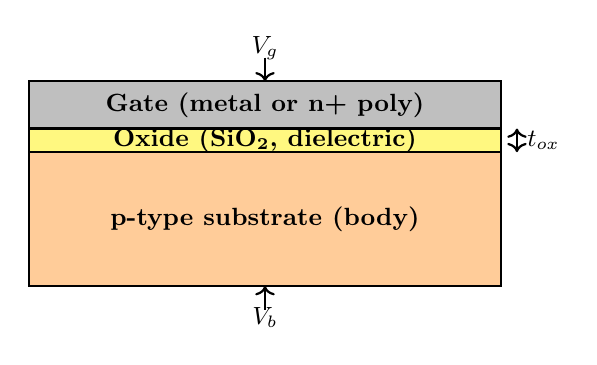
\begin{tikzpicture}[font=\small]
  \fill[gray!50]   (0,2) rectangle (6,2.6);
  \fill[yellow!50] (0,1.7) rectangle (6,2);
  \fill[orange!40] (0,0) rectangle (6,1.7);
  \draw[thick] (0,0) rectangle (6,2.6);
  \draw[thick] (0,2) -- (6,2);
  \draw[thick] (0,1.7) -- (6,1.7);
  \node at (3,2.3) {\textbf{Gate (metal or n+ poly)}};
  \node at (3,1.85) {\textbf{Oxide (SiO\textsubscript{2}, dielectric)}};
  \node at (3,0.85) {\textbf{p-type substrate (body)}};
  \draw[<->,thick] (6.2,1.7) -- (6.2,2) node[midway,right] {$t_{ox}$};
  \draw[->,thick] (3,2.9) -- (3,2.6) node[above=4pt] {$V_g$};
  \draw[->,thick] (3,-0.3) -- (3,0) node[below=4pt] {$V_b$};
\end{tikzpicture}
\\
{\small Figure 1: The MOS capacitor. A parallel-plate capacitor with a metal top plate, an oxide dielectric, and a semiconductor bottom plate.}
\end{center}

That is genuinely it. Three layers. Two terminals. We are going to spend the next thirty pages building everything else on top of this picture.

\subsection{The capacitance formula}

You know parallel-plate caps from intro physics:
\begin{equation}
C_{ox} \;=\; \frac{\varepsilon_{ox}}{t_{ox}}, \qquad \varepsilon_{ox} \approx 3.9\,\varepsilon_0
\end{equation}

Two terms. $\varepsilon_{ox}$ is set by the material (silicon dioxide, in the classical case). $t_{ox}$ is set by the process. As an engineer, you cannot change $\varepsilon_{ox}$ much (changing it is what high-$\kappa$ dielectrics like HfO\textsubscript{2} are for). What you can change is $t_{ox}$.

\subsubsection{Why thinner oxide = stronger transistor (the full chain)}

Let's unpack this carefully, because the chain ``thinner oxide $\Rightarrow$ stronger transistor'' is the entire engine behind two decades of Moore's law and a question you might get asked in an interview.

\paragraph{Move 1: the gate stack is literally a capacitor.} Two conducting plates (the gate on top, the silicon underneath) separated by an insulator (the oxide). That is the textbook definition of a parallel-plate capacitor, so everything you already know about caps applies here.

\paragraph{Move 2: voltage across a cap creates an electric field.} For a parallel-plate capacitor, the field between the plates is:
\begin{equation}
E \;=\; \frac{V}{d}
\end{equation}
where $V$ is the applied voltage and $d$ is the distance between the plates. In our case $d = t_{ox}$.

So if you apply $V_g = 1\,\text{V}$ across a $5\,\text{nm}$ oxide, you get $E = 1\,\text{V}/5\,\text{nm} = 2\times 10^8\,\text{V/m}$. Apply the same $V_g = 1\,\text{V}$ across a $1\,\text{nm}$ oxide and you get $E = 1\times 10^9\,\text{V/m}$. \textbf{Five times stronger field for the same applied voltage.}

\paragraph{Move 3: stronger field pulls in more charge.} A capacitor stores charge $Q = CV$. Plug in $C = \varepsilon_{ox}/t_{ox}$:
\begin{equation}
Q \;=\; \frac{\varepsilon_{ox}}{t_{ox}}\,V
\end{equation}
Cut $t_{ox}$ in half and $Q$ doubles for the same $V$. Cut it to a fifth and $Q$ goes up $5\times$. More induced charge in the silicon surface per volt of gate drive.

In MOSFET language, that induced charge is exactly the channel charge $Q_{inv} = C_{ox}(V_{gs} - V_t)$. Same equation, MOSFET-flavored.

\paragraph{Move 4: more channel charge means more current.} Drain current scales linearly with channel charge:
\begin{equation}
I_d \;=\; Q_{inv} \cdot v
\end{equation}
(charge per unit area times drift velocity). Double the charge and you double the current at the same $V_{ds}$.

\paragraph{The whole chain in one breath.}
\begin{align*}
&\text{thinner } t_{ox} \;\Rightarrow\; \text{bigger } C_{ox} \;\Rightarrow\; \text{stronger } E \text{ at the surface} \\
&\Rightarrow\; \text{more induced } Q_{inv} \;\Rightarrow\; \text{more } I_d
\end{align*}

That is exactly why Moore's law was, for decades, partially an oxide-thinning story. Each new process node, $t_{ox}$ got a little thinner, $C_{ox}$ got a little bigger, and transistors got a little stronger at the same supply voltage. Free performance, just from making the oxide thinner.

\begin{hook}
$C_{ox}$ is the ``leverage'' the gate has on the channel. Imagine pushing a heavy box across a floor: a long stick (thick oxide) wobbles and barely transfers force. A short stick (thin oxide) transfers force directly. The gate uses $C_{ox}$ the way you use a short stick.
\end{hook}

\paragraph{Where this eventually broke (the high-$\kappa$ punchline).} Around $t_{ox} \approx 1\,\text{nm}$ (roughly three atomic layers of SiO\textsubscript{2}), electrons started quantum-tunneling straight through the oxide. The ``insulator'' stopped insulating. Gate leakage exploded and the chip burned static power for nothing.

The industry's fix was elegant: switch from SiO\textsubscript{2} ($\varepsilon \approx 3.9$) to HfO\textsubscript{2} ($\varepsilon \approx 20$). That higher-$\kappa$ dielectric lets you get the same $C_{ox}$ with a \emph{physically thicker} oxide (roughly $5\times$ thicker for equal capacitance), which kills tunneling without giving up channel control. The phrase ``high-$\kappa$ metal gate'' you see in 45 nm and newer processes means exactly this.

\begin{gut}
Two devices, one with a $1\,\text{nm}$ SiO\textsubscript{2} oxide and one with a $5\,\text{nm}$ HfO\textsubscript{2} oxide. Which has more gate leakage? Which has the bigger $C_{ox}$? (Answer: the thin SiO\textsubscript{2} leaks more by tunneling; the HfO\textsubscript{2} has equal-ish $C_{ox}$ because higher $\varepsilon$ compensates for thickness.)
\end{gut}

\subsection{The asymmetric plates (this is the whole twist)}

Here is where the MOS capacitor stops being a normal cap and starts being interesting.

In a normal parallel-plate capacitor, both plates are metal. You pile charge on one plate, an equal and opposite charge shows up on the other instantly. Boring. Predictable.

The MOS cap is different. The top plate is metal, sure. But the bottom plate is \textbf{silicon}, which is a semiconductor. Silicon does not have a sea of free electrons just sitting there waiting to balance whatever charge you dump on the top plate. Silicon has limited carriers (electrons and holes) and fixed ionized dopants. The amount of charge available on the bottom plate depends on what kind of dopants are there, what bias you applied, and what physical processes (depletion, inversion) the silicon has to go through to produce that charge.

\begin{keyidea}
The MOS capacitor has one ``normal'' plate (the metal) and one ``weird'' plate (the silicon). Every interesting behavior of every MOSFET you will ever analyze comes from that asymmetry.
\end{keyidea}

\begin{hook}
Imagine a glass on a table and a stack of poker chips. The glass is the metal plate: you can put as many chips on it as you want, immediately. The other ``plate'' is a piggy bank with a tiny slot: chips can go in, but only at certain speeds and in certain ways. That's why the MOS capacitor responds differently in different regions.
\end{hook}

\begin{pause}
We just learned: the MOS capacitor is a three-layer stack. Its capacitance per area is $\varepsilon_{ox}/t_{ox}$. Thinner oxide gives a stronger device. One plate is metal, the other is silicon, and that mismatch is what makes everything that follows interesting.
\end{pause}

\begin{checkpoint}
Master the MOS capacitor and the rest of the MOSFET is trivial. The source and drain only exist to inject and collect carriers. They do not change the underlying surface physics. We are going to keep coming back to this.
\end{checkpoint}

\section{Flat Band (the weird starting position)}

\begin{tldr}
\begin{itemize}[leftmargin=*]
\item Even at zero applied gate voltage, the MOS capacitor is not ``at rest.'' The metal and the silicon have different work functions, so charges redistribute when you connect them.
\item The voltage you must apply to actually cancel that built-in bending is called the flat-band voltage, $V_{FB}$.
\item Everything else in this document is measured \emph{relative to} $V_{FB}$. It is the origin of the coordinate system.
\end{itemize}
\end{tldr}

\subsection{Zero bias is not zero bending}

You might think: ``If $V_g = V_b = 0$, the cap is just sitting there doing nothing, right?'' No. Even at zero applied voltage, things are happening.

The reason is work functions. The metal in your gate has a specific energy needed to free an electron to vacuum (its work function, $\Phi_M$). The silicon has a different work function ($\Phi_S$). When you connect them through any external wire, electrons spontaneously flow from one to the other until their Fermi levels align.

That redistribution leaves charge sitting around: some on the metal side, some in the silicon. The silicon's energy bands end up \emph{bent} at the surface, even with no externally applied bias.

\subsection{$V_{FB}$ is the cancellation voltage}

To actually flatten those bands (so the silicon surface looks identical to the silicon bulk), you have to apply a specific gate voltage that cancels the built-in offset. That voltage is the \textbf{flat-band voltage}:
\begin{equation}
V_{FB} \;=\; \Phi_{MS} \;-\; \frac{Q_{ox}}{C_{ox}}
\end{equation}
where $\Phi_{MS}$ is the metal-to-semiconductor work-function difference and $Q_{ox}$ is any leftover parasitic charge trapped in the oxide.

You don't need to memorize the formula. You need to memorize the \textbf{concept}.

\begin{keyidea}
$V_{FB}$ is the gate voltage at which the silicon surface looks electrically indistinguishable from the silicon bulk. It is not zero. It is set by materials and process, not by you. All future biasing language ($V_g > 0$, $V_g < V_t$, etc.) implicitly takes $V_{FB}$ as the origin.
\end{keyidea}

\begin{hook}
$V_{FB}$ is like the calibration zero on a kitchen scale. You put an empty bowl on the scale, hit ``tare,'' and now the scale says zero with the bowl still there. The bowl never went away. You just shifted your reference so the math is easier. That is what $V_{FB}$ does for the MOS capacitor.
\end{hook}

When the VLSI Academy lecturer in the video says ``$V_g < 0$,'' he is implicitly working in a coordinate system where $V_{FB} = 0$. The physics is identical to the real case; you just slide the origin. We will follow his convention from now on.

\begin{gut}
If two MOS devices have different gate materials (say, n+ poly vs metal), do they have the same $V_{FB}$? (Answer: no, because $\Phi_M$ is different.)
\end{gut}

\section{The Three Modes (the heart of Lec 3)}

\begin{tldr}
\begin{itemize}[leftmargin=*]
\item Sweep the gate voltage on a MOS capacitor and the silicon surface goes through three distinct physical states: accumulation, depletion, and inversion.
\item The transitions happen at $V_{FB}$ (accumulation to depletion) and at the threshold voltage $V_t$ (depletion to inversion).
\item In accumulation the surface has extra majority carriers. In depletion it has no mobile carriers, just fixed ions. In inversion it has extra minority carriers, which form the conducting channel.
\item NMOS is OFF in accumulation and depletion. NMOS turns ON only once the surface is inverted.
\end{itemize}
\end{tldr}

\subsection{The single rule that explains everything}

Here is the rule. It is so simple it feels like cheating.

\begin{keyidea}
The gate's electric field reaches through the oxide and either attracts or repels mobile charges in the silicon surface. The sign of $V_g - V_{FB}$ tells you which.
\end{keyidea}

That's it. That is the whole engine. The rest is just bookkeeping: as the gate voltage changes, which carriers move where, and what state does the surface end up in?

The substrate is p-type, so it is full of mobile holes (majority carriers) and almost no mobile electrons (minority carriers, present in tiny numbers because of thermal generation). When the gate gets negative, holes get pulled in. When the gate gets positive, holes get pushed away. When the gate gets really positive, electrons start showing up where there used to be none.

\begin{pause}
Three things to keep in your head before we look at the three modes one by one: (1) the gate's field is the cause, (2) the silicon's mobile charges are what respond, and (3) the substrate is p-type so it starts with holes as majority and electrons as minority.
\end{pause}

\subsection{Mode 1: Accumulation ($V_g < V_{FB}$)}

\subsubsection{The story}

You make the gate negative. Negative charge sits on the metal plate. By Coulomb's law that negative charge \emph{attracts} positive charges in the silicon. The silicon already has positive charges available: the holes.

Holes from across the bulk migrate toward the surface and pile up directly under the oxide. The accumulation of majority carriers near the surface is exactly why this mode is called \textbf{accumulation}.

\begin{center}
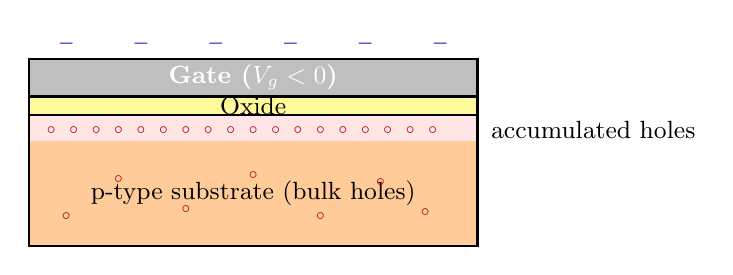
\begin{tikzpicture}[font=\small, scale=0.95]
  \fill[gray!50]   (0,2) rectangle (6,2.5);
  \fill[yellow!40] (0,1.75) rectangle (6,2);
  \fill[red!10]    (0,1.4) rectangle (6,1.75);
  \fill[orange!40] (0,0) rectangle (6,1.4);
  \draw[thick] (0,0) rectangle (6,2.5);
  \draw[thick] (0,2) -- (6,2);
  \draw[thick] (0,1.75) -- (6,1.75);
  \node[white] at (3,2.25) {\textbf{Gate ($V_g < 0$)}};
  \node at (3,1.875) {Oxide};
  \foreach \x in {0.3,0.6,...,5.7} {
    \node[red!70!black] at (\x,1.55) {\tiny $\circ$};
  }
  \node[right] at (6.05,1.55) {\small accumulated holes};
  \node at (3,0.7) {\small p-type substrate (bulk holes)};
  \foreach \x/\y in {0.5/0.4,1.2/0.9,2.1/0.5,3.0/0.95,3.9/0.4,4.7/0.85,5.3/0.45} {
    \node[red!70!black] at (\x,\y) {\tiny $\circ$};
  }
  \foreach \x in {0.5,1.5,...,5.5} {
    \node[blue!70!black] at (\x,2.7) {\scriptsize $-$};
  }
\end{tikzpicture}
\\
{\small Figure 2: Accumulation mode. The negative gate attracts holes to the surface, forming a thin sheet of accumulated majority carriers.}
\end{center}

\subsubsection{What this means for the device}

The surface now has way more holes than the bulk does. Charge balance is straightforward: the negative charge on the gate is exactly cancelled by the positive charge of the accumulated holes. The total capacitance you would measure equals $C_{ox}$, because the accumulated holes behave like a conducting sheet (a near-metal).

In energy-band language, the valence band bends \emph{up} at the surface (closer to the Fermi level means more holes). We will not dwell on band diagrams here, but file that away.

\subsubsection{Is the NMOS on?}

Nope. Hard off. Here is why. The source and drain are n+ regions, which are full of electrons. Current in an NMOS is supposed to flow as electrons through a channel under the gate. But the gate just attracted a giant pile of \emph{holes} to the surface. That is the opposite of a channel for electrons. The electrons in the source cannot push through a hole-rich surface. The device is solidly off.

\begin{hook}
Accumulation = ``gate attracts the wrong team.'' You wanted electrons under the gate to make a channel. Instead, you piled up holes. Holes block the channel. Game over.
\end{hook}

\begin{gut}
For a PMOS (n-type substrate), would accumulation happen at $V_g > 0$ or $V_g < 0$? (Answer: $V_g > 0$, because in n-substrate the majority carriers are electrons, and a \emph{positive} gate would attract them.)
\end{gut}

\subsection{Mode 2: Depletion ($V_{FB} < V_g < V_t$)}

\subsubsection{The story}

Now flip the sign. Make the gate slightly \emph{positive}. The positive charge on the metal plate \textbf{repels} the holes that were sitting at the surface. They migrate back into the bulk.

But wait. Why were holes there in the first place? Because the substrate is p-type, which means it has \textbf{ionized acceptor atoms} (boron). Each boron atom, when ionized, carries a fixed negative charge. In the bulk those fixed negative charges are screened by the mobile holes (electrically the bulk is neutral). When you push the holes away from the surface, you expose the fixed negative charges.

The region near the surface is now \emph{depleted} of mobile carriers. Only fixed ionized acceptor ions remain. That is why this mode is called \textbf{depletion}.

\subsubsection{The capacitance drops here}

This is one of the things that makes the MOS capacitor weird. As the depletion region grows, you have effectively added a \emph{second capacitor} (the depletion region itself, with its own thickness $W_{dep}$) in series with the oxide capacitor. Two capacitors in series have a total capacitance smaller than either one alone:
\begin{equation}
\frac{1}{C_{\text{total}}} \;=\; \frac{1}{C_{ox}} + \frac{1}{C_{dep}}, \qquad C_{dep} = \frac{\varepsilon_{si}}{W_{dep}}
\end{equation}

So as you sweep $V_g$ from $V_{FB}$ upward, the capacitance you would measure starts dropping below $C_{ox}$. This dip in capacitance is the signature of being in depletion. You will see it on the C to V curve in a bit.

\subsubsection{Is the NMOS on?}

Still nope. There are no mobile electrons at the surface yet. Just fixed ions. The source and drain still cannot find a path to push electrons through. The NMOS is still off.

\begin{hook}
Depletion = ``nothing's home.'' You evicted the holes. The electrons haven't moved in yet. The surface is a ghost town of bare acceptor ions. Nothing conducts.
\end{hook}

\begin{pitfall}
The video glosses over a subtle but \emph{critical} reality. Between depletion and strong inversion there is a regime called \textbf{weak inversion} or \textbf{subthreshold}, where minority carriers start showing up at the surface in exponentially increasing numbers below the textbook threshold voltage. Current actually flows in subthreshold, just exponentially small. This is the primary source of static power in modern chips. We come back to it in Section~\ref{sec:subthreshold}. For now, just know that ``depletion = perfectly off'' is a useful simplification, not the full truth.
\end{pitfall}

\subsection{Mode 3: Strong Inversion ($V_g > V_t$)}

\subsubsection{The story}

Push $V_g$ further positive. At some point, the gate is positive enough that it doesn't just repel holes anymore. It starts \emph{attracting electrons} from the bulk to the surface.

Now, the p-substrate has very few electrons (they are the minority carriers). But ``very few'' isn't zero. There are always some, generated thermally. As $V_g$ rises, those rare electrons get pulled to the surface and pile up under the oxide.

When the gate gets positive enough, you reach the magic moment: the surface has so many electrons that it looks more n-type than the bulk looks p-type. The surface has been \textbf{inverted}. A p-substrate now has an n-type surface layer.

\subsubsection{The formal condition: $\psi_s = 2\phi_F$}

The textbook definition of strong inversion uses two symbols you will see in any device-physics class. $\psi_s$ is the \textbf{surface potential}: how much the bands have bent at the surface. $\phi_F$ is the \textbf{bulk Fermi potential}: how far below mid-gap the Fermi level sits in the p-bulk.

When $\psi_s = 2\phi_F$, the electron concentration at the surface equals the hole concentration in the bulk. That is, by definition, the moment ``the surface is as n-type as the bulk is p-type.''

The gate voltage at which this happens is the threshold voltage, $V_t$. We will derive $V_t$ in the next section.

\subsubsection{Is the NMOS on?}

YES. Finally. The inversion layer is a thin n-type channel connecting the n+ source to the n+ drain. Apply $V_{ds} > 0$, electrons drift from source to drain, current flows. The MOSFET conducts.

\begin{hook}
Inversion = ``the gate built a bridge.'' Source and drain are two islands of electrons. The p-substrate between them is a moat of holes. When you crank the gate, the surface flips polarity and becomes an electron bridge connecting the islands.
\end{hook}

\begin{pause}
Three modes, three states, three colors of physics. Accumulation: too many of the wrong team (holes). Depletion: nobody's home (just fixed ions). Inversion: the right team showed up (electrons), the bridge is built, current flows.
\end{pause}

\subsection{Band diagrams across the three modes}

A picture is worth a thousand words. Energy-band sketches for the three modes, conduction band $E_c$ on top and valence band $E_v$ on bottom, Fermi level $E_F$ as the dashed reference:

\begin{center}
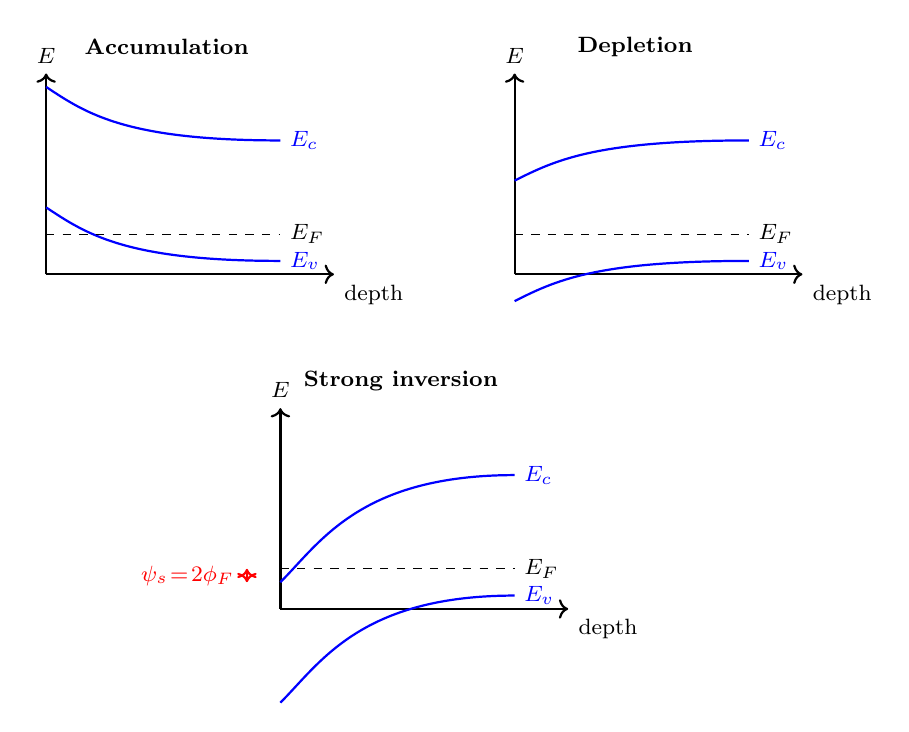
\begin{tikzpicture}[font=\footnotesize, scale=0.85]
  % Accumulation
  \begin{scope}[xshift=0cm]
    \draw[->,thick] (0,0) -- (4.3,0) node[below right] {depth};
    \draw[->,thick] (0,0) -- (0,3) node[above] {$E$};
    \draw[thick,blue] (0,2.8) .. controls (0.6,2.4) and (1.2,2) .. (3.5,2);
    \draw[thick,blue] (0,1.0) .. controls (0.6,0.6) and (1.2,0.2) .. (3.5,0.2);
    \draw[dashed] (0,0.6) -- (3.5,0.6);
    \node at (1.8,3.4) {\textbf{Accumulation}};
    \node[blue,right] at (3.5,2) {$E_c$};
    \node[right] at (3.5,0.6) {$E_F$};
    \node[blue,right] at (3.5,0.2) {$E_v$};
  \end{scope}
  % Depletion
  \begin{scope}[xshift=7cm]
    \draw[->,thick] (0,0) -- (4.3,0) node[below right] {depth};
    \draw[->,thick] (0,0) -- (0,3) node[above] {$E$};
    \draw[thick,blue] (0,1.4) .. controls (0.6,1.7) and (1.2,2) .. (3.5,2);
    \draw[thick,blue] (0,-0.4) .. controls (0.6,-0.1) and (1.2,0.2) .. (3.5,0.2);
    \draw[dashed] (0,0.6) -- (3.5,0.6);
    \node at (1.8,3.4) {\textbf{Depletion}};
    \node[blue,right] at (3.5,2) {$E_c$};
    \node[right] at (3.5,0.6) {$E_F$};
    \node[blue,right] at (3.5,0.2) {$E_v$};
  \end{scope}
  % Inversion (next row)
  \begin{scope}[xshift=3.5cm,yshift=-5cm]
    \draw[->,thick] (0,0) -- (4.3,0) node[below right] {depth};
    \draw[->,thick] (0,0) -- (0,3) node[above] {$E$};
    \draw[thick,blue] (0,0.4) .. controls (0.6,1.0) and (1.2,2) .. (3.5,2);
    \draw[thick,blue] (0,-1.4) .. controls (0.6,-0.8) and (1.2,0.2) .. (3.5,0.2);
    \draw[dashed] (0,0.6) -- (3.5,0.6);
    \node at (1.8,3.4) {\textbf{Strong inversion}};
    \node[blue,right] at (3.5,2) {$E_c$};
    \node[right] at (3.5,0.6) {$E_F$};
    \node[blue,right] at (3.5,0.2) {$E_v$};
    \draw[<->,thick,red] (-0.5,0.4) -- (-0.5,0.6);
    \node[red,left] at (-0.55,0.5) {$\psi_s\!=\!2\phi_F$};
  \end{scope}
\end{tikzpicture}
\\
{\small Figure 3: Band bending at the silicon surface across the three modes. In accumulation the valence band bends up toward $E_F$ (more holes). In depletion the bands bend down a little (carriers leaving). In inversion the bands bend so far that the conduction band approaches $E_F$ at the surface (electron sheet forms).}
\end{center}

\subsection{Mode 3 (Strong Inversion) picture}

\begin{center}
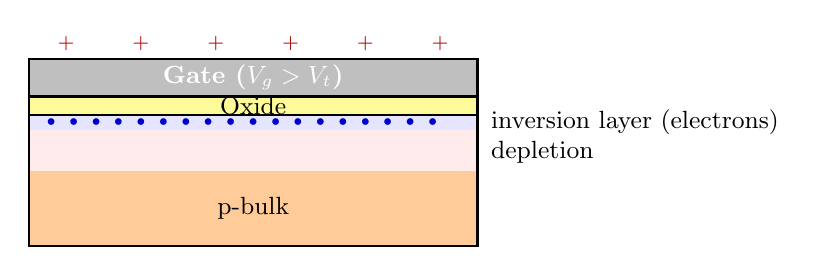
\begin{tikzpicture}[font=\small, scale=0.95]
  \fill[gray!50]   (0,2) rectangle (6,2.5);
  \fill[yellow!40] (0,1.75) rectangle (6,2);
  \fill[blue!10]   (0,1.55) rectangle (6,1.75);
  \fill[red!8]     (0,1.0) rectangle (6,1.55);
  \fill[orange!40] (0,0) rectangle (6,1.0);
  \draw[thick] (0,0) rectangle (6,2.5);
  \draw[thick] (0,2) -- (6,2);
  \draw[thick] (0,1.75) -- (6,1.75);
  \node[white] at (3,2.25) {\textbf{Gate ($V_g > V_t$)}};
  \node at (3,1.875) {Oxide};
  \foreach \x in {0.3,0.6,...,5.7} {
    \node[blue!80!black] at (\x,1.65) {\tiny $\bullet$};
  }
  \node[right] at (6.05,1.65) {\small inversion layer (electrons)};
  \node[right] at (6.05,1.25) {\small depletion};
  \node at (3,0.5) {\small p-bulk};
  \foreach \x in {0.5,1.5,...,5.5} {
    \node[red!70!black] at (\x,2.7) {\scriptsize $+$};
  }
\end{tikzpicture}
\\
{\small Figure 4: Strong inversion. The gate has attracted enough electrons to the surface to form an n-type channel. Below it sits a maximum-width depletion region.}
\end{center}

\subsection{The mnemonic to never forget the order}

If you ever blank on which mode comes first, just remember the sweep direction for NMOS:
\[
\boxed{\text{negative } V_g \;\to\; \text{slightly positive } V_g \;\to\; \text{very positive } V_g}
\]
\[
\downarrow \qquad\qquad \downarrow \qquad\qquad \downarrow
\]
\[
\text{ACCUMULATION} \;\to\; \text{DEPLETION} \;\to\; \text{INVERSION}
\]

For PMOS, flip everything. Sweep from positive to negative; same three modes in the same order, but the carrier species swap.

\begin{checkpoint}
The three modes are three physical states of the silicon surface as $V_g$ varies. The gate's field attracts or repels mobile charges. Holes flood in (accumulation), holes flee leaving bare ions (depletion), electrons flood in (inversion). The first two states leave the NMOS off. The third turns it on.
\end{checkpoint}

\section{Threshold Voltage From First Principles}
\label{sec:vt}

\begin{tldr}
\begin{itemize}[leftmargin=*]
\item Threshold voltage $V_t$ is the gate voltage at which the surface just barely reaches strong inversion.
\item The formula has three additive pieces: a flat-band term, a surface-bending term, and a depletion-charge term.
\item Each piece has a physical meaning you can recite in one sentence.
\item $V_t$ depends on doping, on oxide thickness, and on body bias. All three of those are levers PD engineers use indirectly through cell-library choices.
\end{itemize}
\end{tldr}

\subsection{The formula you must be able to recite cold}

\begin{equation}
\boxed{V_t \;=\; V_{FB} \;+\; 2\phi_F \;+\; \frac{\sqrt{2q\varepsilon_{si} N_A (2\phi_F)}}{C_{ox}}}
\end{equation}

It looks intimidating until you decompose it. Three terms. Each one is doing one job.

\subsection{Term 1: $V_{FB}$, the cost of getting to flat}

Before you can bend any bands intentionally, you have to undo the built-in bending that came from work-function mismatch. That undoing costs $V_{FB}$. It is the ``you can't start at zero, you start at $V_{FB}$'' tax.

\subsection{Term 2: $2\phi_F$, the cost of inverting the surface}

Now that the bands are flat, you have to bend them by $2\phi_F$ at the surface to flip the polarity. Bend less and the surface is just depleted; bend by exactly $2\phi_F$ and you have created strong inversion. This is the ``flip the surface tax.''

\subsection{Term 3: depletion-charge term, the cost of supporting the ions}

When you bend the bands to invert the surface, you also expose a maximum-width depletion region full of fixed acceptor ions. The gate has to electrostatically support all that fixed charge across the oxide capacitance. That is what the gnarly square-root term represents: the gate voltage equivalent of holding up $Q_{dep,max}$ across $C_{ox}$.

\begin{hook}
Think of $V_t$ as the tab at the end of a meal with three line items.
\begin{itemize}
\item Cover charge for the work-function mismatch: $V_{FB}$.
\item Entr\'ee of bending the bands enough to invert the surface: $2\phi_F$.
\item Side dish of holding the depletion charge up across $C_{ox}$: the square-root term.
\end{itemize}
Pay all three and the surface is on the edge of strong inversion. That total is what you call $V_t$.
\end{hook}

\subsection{Three consequences that matter for PD work}

The formula tells you exactly which knobs change $V_t$.

\subsubsection{$V_t$ depends on channel doping ($N_A$)}

Higher channel doping makes the third term bigger, which raises $V_t$. Higher $V_t$ means a slower transistor (smaller overdrive for the same supply) but lower leakage.

This is exactly how foundries make \textbf{HVT / SVT / LVT} flavors of the same cell. The layout is identical. The channel implant dose is different. Different implant dose, different $N_A$, different $V_t$.

\subsubsection{$V_t$ depends on oxide thickness ($C_{ox}$)}

A larger $C_{ox}$ (thinner oxide) makes the third term smaller, which lowers $V_t$. This is one of the levers process engineers use to keep $V_t$ controllable as supply voltage scales down.

\subsubsection{$V_t$ depends on body bias ($V_{sb}$)}

If the source is reverse-biased relative to the body ($V_{sb} > 0$), the surface needs to bend even more before reaching strong inversion. The effective $\phi_F$ increases, the depletion charge term grows, and $V_t$ rises:
\begin{equation}
V_t \;=\; V_{t0} \;+\; \gamma\,\Big(\sqrt{2\phi_F + V_{sb}} \;-\; \sqrt{2\phi_F}\Big), \qquad \gamma = \frac{\sqrt{2q\varepsilon_{si}N_A}}{C_{ox}}
\end{equation}

We will treat this in agonizing detail in Part II. For now: stacked transistors have $V_{sb} > 0$ on the upper devices, which makes them weaker than the bottom devices. That is the body effect in one sentence.

\begin{pdnote}
The HVT / SVT / LVT distinction is the most direct application of the $V_t$ formula you will encounter as a PD engineer. During timing closure, you swap critical-path cells to LVT (faster, leakier). During leakage recovery, you swap slack-rich cells to HVT (slower, less leaky). Knowing that ``$V_t$ is set by channel doping and oxide thickness'' makes those swaps feel meaningful instead of like magic.
\end{pdnote}

\begin{checkpoint}
$V_t$ is the gate voltage at which the silicon surface just barely reaches strong inversion. It has three additive parts, each with a physical job. It changes with doping, oxide thickness, and body bias. Foundries exploit the doping dependence to give you HVT, SVT, and LVT cells.
\end{checkpoint}

\subsection{Tiny numerical example}

Let's plug numbers in just so the formula is not abstract.

Assume $V_{FB} = -0.9\,\text{V}$ (typical n+ poly gate on p-substrate), $2\phi_F = 0.7\,\text{V}$, $N_A = 5\times 10^{17}\,\text{cm}^{-3}$, $t_{ox} = 2\,\text{nm}$ so $C_{ox} \approx 17.3\,\text{fF}/\mu\text{m}^2$.

The depletion-charge term works out to roughly $0.3\,\text{V}$. Adding it all up:
\[
V_t \;\approx\; -0.9 + 0.7 + 0.3 = 0.1\,\text{V}
\]

That is suspiciously low for a real chip; we'd want $V_t \approx 0.3$ to $0.5\,\text{V}$ for reasonable noise margin and leakage. Foundries use threshold-adjust implants to bring $V_t$ up to where they want it. The point of the calculation is not the exact answer but to see that each of the three terms contributes a substantial amount.

\section{The C to V Curve (the universal diagnostic)}

\begin{tldr}
\begin{itemize}[leftmargin=*]
\item Sweep $V_g$ on a MOS capacitor while measuring its small-signal capacitance, and you get a C to V curve.
\item Three regions: accumulation, depletion, inversion. Each one has a different physical mechanism setting the capacitance.
\item In inversion the curve splits into two: low-frequency (the inversion layer can keep up with AC) and high-frequency (it cannot).
\item Foundries use C to V curves to extract $V_{FB}$, $V_t$, doping, and oxide quality on every wafer. Recognize this curve instantly.
\end{itemize}
\end{tldr}

\subsection{What the measurement looks like}

\begin{center}
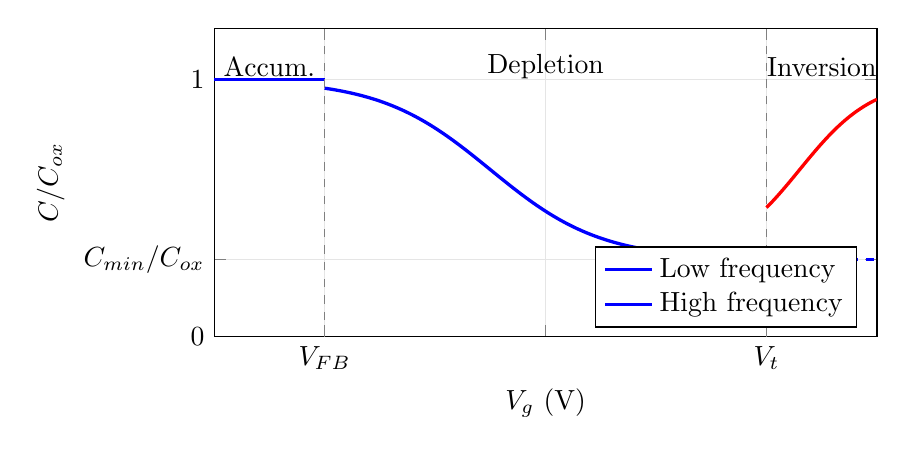
\begin{tikzpicture}
\begin{axis}[
  width=10cm, height=5.5cm,
  xlabel={$V_g$ (V)}, ylabel={$C/C_{ox}$},
  xtick={-2,0,2}, xticklabels={$V_{FB}$,,$V_t$},
  ytick={0,0.3,1}, yticklabels={0,$C_{min}/C_{ox}$,1},
  ymin=0, ymax=1.2, xmin=-3, xmax=3,
  legend pos=south east, legend cell align=left,
  grid=major, grid style={gray!20}
]
% Accumulation/depletion (shared)
\addplot[blue, very thick, domain=-3:-2, samples=20] {1};
\addplot[blue, very thick, domain=-2:2, samples=80] {0.3 + 0.7/(1 + exp(2.0*(x+0.5)))};
% Low frequency in inversion
\addplot[red, very thick, domain=2:3, samples=40] {0.3 + 0.7/(1 + exp(-3*(x-2.3)))};
\addlegendentry{Low frequency}
% High frequency in inversion
\addplot[blue, very thick, dashed, domain=2:3, samples=20] {0.3};
\addlegendentry{High frequency}
% Vertical guides
\draw[gray,dashed] (axis cs:-2,0) -- (axis cs:-2,1.2);
\draw[gray,dashed] (axis cs:2,0) -- (axis cs:2,1.2);
\node at (axis cs:-2.5,1.05) {Accum.};
\node at (axis cs:0,1.05) {Depletion};
\node at (axis cs:2.5,1.05) {Inversion};
\end{axis}
\end{tikzpicture}
\\
{\small Figure 5: MOS capacitor C to V curve at low and high measurement frequencies. Read left to right: accumulation, depletion, inversion.}
\end{center}

\subsection{Reading each region}

\subsubsection{Accumulation (left flat region)}

$V_g$ is below $V_{FB}$. The surface has accumulated holes acting as a conducting sheet. The cap behaves like a normal parallel-plate, $C = C_{ox}$. Flat top.

\subsubsection{Depletion (the dip in the middle)}

$V_g$ is between $V_{FB}$ and $V_t$. The depletion region has thickness, which adds a series capacitance below $C_{ox}$. As $V_g$ rises, $W_{dep}$ grows, $C_{dep}$ shrinks, and the total capacitance drops. This is the downward slope.

\subsubsection{Inversion (right side, two curves)}

Here is the weird part. The inversion layer can supply or absorb charge as the small-signal AC voltage wiggles up and down, \emph{but only if the AC is slow enough that minority carriers can be generated and recombined in time}. So:
\begin{itemize}
\item \textbf{Low-frequency curve}: the inversion layer keeps up. The cap returns to $C_{ox}$.
\item \textbf{High-frequency curve}: the inversion layer can't keep up. Only the depletion region responds. The cap stays low.
\end{itemize}

\begin{hook}
Inversion-layer frequency response is like a slow waiter at a busy restaurant. At low frequency (one table at a time), the waiter handles every order. At high frequency (everyone ordering at once), the waiter falls behind and most tables get ignored. The orders the waiter does reach correspond to the depletion region (which is fast); the inversion layer is the slow waiter.
\end{hook}

\begin{keyidea}
The C to V curve is the universal diagnostic of a MOS process. From it you can extract $V_{FB}$ (where the cap starts dropping), $V_t$ (where the cap bottoms out), doping (from the depth of the dip), and oxide quality (from how clean the curve looks). Every foundry runs this on every wafer.
\end{keyidea}

\begin{gut}
If you saw a C to V curve where the inversion side stayed at exactly $C_{ox}$, would you guess that was measured at low or high frequency? (Answer: low.)
\end{gut}

\section{From MOS Capacitor to MOSFET}

\begin{tldr}
\begin{itemize}[leftmargin=*]
\item Take a MOS capacitor and add two heavily-doped n+ regions on either side: those are the source and drain.
\item Their only job is to inject and collect electrons at low resistance.
\item They do not change the surface physics under the gate. The MOS capacitor is still in charge.
\item When the surface is inverted, the n+ source and n+ drain are bridged by the n-type channel. Current flows.
\end{itemize}
\end{tldr}

\subsection{Adding source and drain}

We have been studying the gate stack in isolation. Time to add the rest of the device.

\begin{center}
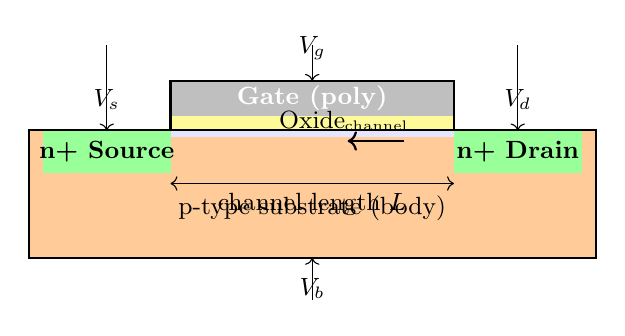
\begin{tikzpicture}[font=\small,scale=0.9]
  \fill[orange!40] (0,0) rectangle (8,1.8);
  \fill[green!40]  (0.2,1.2) rectangle (2.0,1.8);
  \fill[green!40]  (6.0,1.2) rectangle (7.8,1.8);
  \fill[blue!10]   (2.0,1.7) rectangle (6.0,1.8);
  \fill[yellow!40] (2.0,1.8) rectangle (6.0,2.0);
  \fill[gray!50]   (2.0,2.0) rectangle (6.0,2.5);
  \draw[thick] (0,0) rectangle (8,1.8);
  \draw[thick] (2.0,1.8) rectangle (6.0,2.5);
  \node at (1.1,1.5) {\textbf{n+ Source}};
  \node at (6.9,1.5) {\textbf{n+ Drain}};
  \node at (4,1.95) {Oxide};
  \node[white] at (4,2.25) {\textbf{Gate (poly)}};
  \node at (4,0.7) {p-type substrate (body)};
  \draw[<->] (2.0,1.05) -- (6.0,1.05) node[midway,below] {channel length $L$};
  \draw[->] (4,3.0) -- (4,2.5) node[above=4pt] {$V_g$};
  \draw[->] (1.1,3.0) -- (1.1,1.8) node[above=4pt] {$V_s$};
  \draw[->] (6.9,3.0) -- (6.9,1.8) node[above=4pt] {$V_d$};
  \draw[->] (4,-0.6) -- (4,0) node[below=4pt] {$V_b$};
  \draw[->,thick] (5.3,1.65) -- (4.5,1.65) node[midway,above] {\tiny channel};
\end{tikzpicture}
\\
{\small Figure 6: NMOS cross section. Two heavily-doped n+ regions flank the gate. The gate, oxide, and substrate still form a MOS capacitor. When inverted, the channel bridges source to drain.}
\end{center}

\subsection{What the source and drain are actually for}

You might be tempted to think the source and drain are doing something deep. They're not. Their job is simple.

\begin{itemize}
\item The \textbf{source} is a reservoir of electrons. When the channel is on, the source can supply as many electrons as the channel can carry, with negligible resistance.
\item The \textbf{drain} is a sink for electrons. They flow into it and out to the external circuit.
\end{itemize}

That's the whole story. The source and drain are heavily doped n+ specifically so they have lots of electrons and very low resistivity. They are passive endpoints. They do not change the physics of the surface under the gate.

\begin{keyidea}
The source and drain just give you a way to detect (as a current) whether the gate succeeded in building a channel. The MOS capacitor we spent the last twenty pages on is still the protagonist.
\end{keyidea}

\subsection{The channel sits at the surface}

Notice in the figure that the channel (drawn faded blue) sits at the very top of the substrate, right under the oxide. That's not artistic license. The inversion layer is genuinely a thin sheet right at the silicon-oxide interface, typically only a few nanometers thick. The gate's electric field is strongest at the surface and falls off into the bulk. So the inversion only happens at the surface.

\begin{gut}
If the inversion layer is only a few nm thick but the substrate is hundreds of nm thick, where does the current actually flow? (Answer: only at the surface. The bulk is irrelevant for source-to-drain current.)
\end{gut}

\section{Channel Charge and Drain Current}

\begin{tldr}
\begin{itemize}[leftmargin=*]
\item Once the surface is inverted, every extra volt of $V_{gs}$ above $V_t$ adds more channel charge: $Q_{inv} = C_{ox}(V_{gs} - V_t)$.
\item The quantity $V_{gs} - V_t$ is the overdrive voltage, $V_{ov}$. Burn this term into your head. It's everywhere.
\item Triode region ($V_{ds} < V_{ov}$): the transistor acts like a resistor whose value is set by $V_{ov}$.
\item Saturation region ($V_{ds} \ge V_{ov}$): the channel pinches off at the drain end, $I_d$ becomes nearly independent of $V_{ds}$, and $I_d \propto V_{ov}^2$.
\end{itemize}
\end{tldr}

\subsection{Where $Q_{inv} = C_{ox}(V_{gs} - V_t)$ comes from}

In strong inversion, the depletion charge under the gate is essentially maxed out (it cannot grow much more). So every additional volt of $V_{gs}$ above $V_t$ has to be supported by \emph{additional channel charge}, not additional depletion charge.

By charge balance on the MOS capacitor:
\begin{equation}
\boxed{Q_{inv} \;=\; C_{ox}\,(V_{gs} - V_t)}
\end{equation}

This is called the \textbf{charge-sheet model} or the \textbf{strong-inversion approximation}. It says: the inversion charge is exactly the gate overdrive times the oxide capacitance. Crisp, clean, useful.

\begin{pitfall}
This is an approximation. It assumes (a) the inversion layer is infinitely thin (which it isn't, it's a few nm thick), and (b) there is no current below $V_t$ (which is wrong; that's subthreshold leakage). For hand analysis it's excellent. For real circuit simulation, BSIM models replace it with much fancier expressions.
\end{pitfall}

\subsection{Why $V_{ov}$ is the most important number}

The overdrive voltage $V_{ov} \equiv V_{gs} - V_t$ shows up in every MOSFET equation you'll ever write. Drain current, on-resistance, transconductance, output resistance, saturation voltage: all of them are expressed in terms of $V_{ov}$.

\begin{keyidea}
If someone wakes you up at 3am and asks ``what's $V_{ov}$?'', you should be able to say ``how much the gate voltage exceeds threshold, $V_{gs} - V_t$'' before you're even fully conscious. Then go back to sleep.
\end{keyidea}

\subsection{The two regions}

When you apply a drain voltage $V_{ds}$, the channel responds. Depending on how big $V_{ds}$ is relative to $V_{ov}$, you get one of two regimes.

\subsubsection{Triode region (also called linear or ohmic)}

\textbf{Condition:} $V_{ds} < V_{ov}$.

The channel exists end-to-end from source to drain. Electrons drift through it. For small $V_{ds}$ the device looks like a resistor:
\begin{equation}
R_{on} \;\approx\; \frac{1}{\mu_n C_{ox}\,\frac{W}{L}\,(V_{gs}-V_t)}
\end{equation}

For larger $V_{ds}$ (still in triode), the drain current has a quadratic correction:
\begin{equation}
I_d \;=\; \mu_n C_{ox}\,\frac{W}{L}\,\left[(V_{gs}-V_t)V_{ds} \;-\; \frac{V_{ds}^2}{2}\right]
\end{equation}

\begin{hook}
Triode = ``it's a knob.'' $R_{on}$ is your knob, $V_{ov}$ turns it. This is exactly how pass-gates, transmission gates, and analog switches work. You don't bias them in saturation; you keep them in triode and treat them as voltage-controlled resistors.
\end{hook}

\subsubsection{Saturation region (also called active)}

\textbf{Condition:} $V_{ds} \ge V_{ov}$.

The channel ``pinches off'' at the drain end (we'll explain in Part II). Above that, raising $V_{ds}$ doesn't add more current to first order. The current saturates at:
\begin{equation}
I_d \;=\; \tfrac{1}{2}\,\mu_n C_{ox}\,\frac{W}{L}\,(V_{gs}-V_t)^2\,(1 + \lambda V_{ds})
\end{equation}

The $(1 + \lambda V_{ds})$ factor is channel-length modulation (Part II). For ideal long-channel devices, $\lambda \approx 0$ and the term vanishes.

\begin{hook}
Saturation = ``it's a current source.'' $I_d$ depends on $V_{ov}$ and almost nothing else. Every analog gain stage, every current mirror, every active load lives here.
\end{hook}

\subsection{The classic I to V family}

\begin{center}
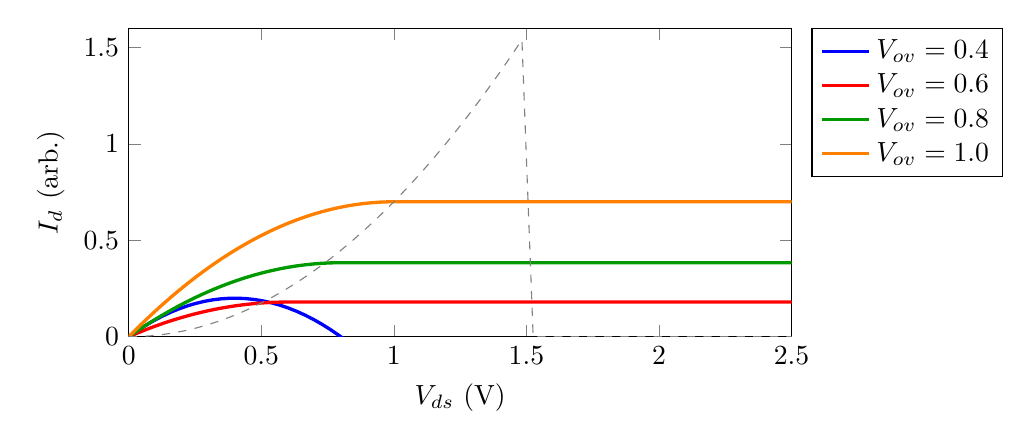
\begin{tikzpicture}
\begin{axis}[
  width=10cm, height=5.5cm,
  xlabel={$V_{ds}$ (V)}, ylabel={$I_d$ (arb.)},
  xmin=0, xmax=2.5, ymin=0, ymax=1.6,
  legend pos=outer north east, legend cell align=left,
  domain=0:2.5, samples=80
]
\addplot[blue, very thick] {min(x/0.4 - 0.5*(x/0.4)^2, 0.5)*0.4};
\addlegendentry{$V_{ov}=0.4$}
\addplot[red, very thick] {min(0.6*x - 0.5*x*x*((x<0.6)+(x>=0.6)*(0.6/x)), 0.18)*1.0+0.05*(x>0.6)*0};
\addlegendentry{$V_{ov}=0.6$}
\addplot[green!60!black, very thick] {min(0.8*x - 0.5*x*x*((x<0.8)+(x>=0.8)*(0.8/x)), 0.32)*1.2};
\addlegendentry{$V_{ov}=0.8$}
\addplot[orange, very thick] {min(1.0*x - 0.5*x*x*((x<1.0)+(x>=1.0)*(1.0/x)), 0.5)*1.4};
\addlegendentry{$V_{ov}=1.0$}
\addplot[dashed, gray, samples=60] {0.7*x*x*(x<1.5)};
\end{axis}
\end{tikzpicture}
\\
{\small Figure 7: Family of $I_d$ vs $V_{ds}$ curves at different gate overdrives. The dashed parabola separates triode (current rising) from saturation (current nearly flat).}
\end{center}

\subsection{Worked example: just the math, on paper}

\textbf{Setup.} $\mu_n C_{ox} = 200\,\mu\text{A}/\text{V}^2$. $W/L = 4$. $V_{gs} = 1.0\,\text{V}$. $V_t = 0.4\,\text{V}$. So $V_{ov} = 0.6\,\text{V}$.

\textbf{Compute $R_{on}$ at $V_{ds}$ near zero.}
\[
R_{on} \;=\; \frac{1}{200\,\mu\text{A}/\text{V}^2 \cdot 4 \cdot 0.6\,\text{V}} \;\approx\; 2.08\,\text{k}\Omega
\]

\textbf{Compute $I_d$ in saturation at $V_{ds} = 1\,\text{V}$, assuming $\lambda = 0$.}
\[
I_d = \tfrac{1}{2} \cdot 200\,\mu\text{A}/\text{V}^2 \cdot 4 \cdot (0.6)^2 = 144\,\mu\text{A}
\]

That's it. Two equations, two numbers. The triode equation gives you a resistance; the saturation equation gives you a current. Practice plugging in until it feels automatic.

\begin{checkpoint}
Three things to carry forever. (1) $V_{ov} = V_{gs} - V_t$, the gate overdrive. (2) In triode, $R_{on} \propto 1/V_{ov}$, the device is a resistor. (3) In saturation, $I_d \propto V_{ov}^2$, the device is a current source. Master the regime check ($V_{ds}$ vs $V_{ov}$) and you can plug into the right equation every time.
\end{checkpoint}

\section{PMOS (the mirror)}

\begin{tldr}
\begin{itemize}[leftmargin=*]
\item PMOS is the symmetric mirror of NMOS: n-type substrate, p+ source and drain, channel made of holes.
\item All signs flip. Threshold is negative. PMOS turns on when $V_{gs}$ is sufficiently negative ($V_{sg} > |V_{tp}|$).
\item Holes are slower than electrons by about $2.5\times$, so PMOS is drawn wider than NMOS for matching drive.
\item CMOS works because in any static state, exactly one of NMOS / PMOS conducts. That's zero static current. That's the whole game.
\end{itemize}
\end{tldr}

\subsection{The mirror table}

\begin{center}
\begin{tabular}{lll}
\toprule
Property & NMOS & PMOS \\
\midrule
Substrate (well) & p-type (bulk holes) & n-type (bulk electrons) \\
S / D regions & n+ (electron rich) & p+ (hole rich) \\
Channel carriers & Electrons & Holes \\
Threshold voltage & $V_{tn} > 0$ & $V_{tp} < 0$ \\
On condition & $V_{gs} > V_{tn}$ & $V_{gs} < V_{tp}$, i.e., $V_{sg} > |V_{tp}|$ \\
Source connected to & $V_{ss}$ (GND) & $V_{dd}$ \\
Carrier mobility & $\mu_n$ (higher) & $\mu_p \approx 0.4\,\mu_n$ \\
\bottomrule
\end{tabular}
\\
{\small Table 1: NMOS vs PMOS at a glance.}
\end{center}

\subsection{Why CMOS works (the punchline of CMOS)}

In a static CMOS gate, the PMOS pull-up network is on when the input is logic 0. The NMOS pull-down network is on when the input is logic 1. \textbf{Exactly one of them conducts in any static state.} The other is off.

That means in any static state, there is no DC path from $V_{dd}$ to ground. Zero static current. That is the entire reason CMOS dominated every other logic family for static digital design.

\begin{keyidea}
CMOS is not a clever choice. It's the only logic family that fundamentally cannot burn static power, because the complementary structure guarantees one network is always off. Everything else (NMOS-only, PMOS-only, BiCMOS) has DC current paths and pays a constant power tax.
\end{keyidea}

\subsection{Why PMOS is drawn wider}

Hole mobility is about $2.5\times$ smaller than electron mobility. To match the drive current of an NMOS, you need to scale the PMOS up by roughly that ratio. Look at any standard cell layout in a foundry library and you'll see the PMOS rows are $2\times$ to $2.5\times$ taller than the NMOS rows.

\begin{gut}
If you're designing an inverter and you want it to switch symmetrically (the rising edge takes the same time as the falling edge), what should the ratio $W_p/W_n$ be? (Answer: roughly 2 to 2.5, matching the mobility ratio.)
\end{gut}

\subsection{The PMOS-off question from the video}

The lecture asks: ``what should $V_g$ be for PMOS to be off?'' Look at the table. PMOS source is at $V_{dd}$. PMOS is off when $V_{sg} < |V_{tp}|$, that is, when the gate is not pulled much below $V_{dd}$. In an inverter, an input of logic 1 (gate at $V_{dd}$) gives $V_{sg} = 0$, which is well below $|V_{tp}|$, so PMOS is fully off.

\begin{checkpoint}
PMOS is NMOS through a mirror. Same physics, all signs flipped, mobility $2.5\times$ slower. CMOS works because complementary networks guarantee zero static current. Width ratios in standard cells compensate for the mobility imbalance.
\end{checkpoint}

\section{What Actually Happens in Real Modern Devices}
\label{sec:subthreshold}

\begin{tldr}
\begin{itemize}[leftmargin=*]
\item Real transistors have subthreshold leakage, drain-induced barrier lowering (DIBL), body effect, and PVT variation. None of those are in the simple model.
\item All of them trace back to the same MOS capacitor physics; they are second-order effects on the same picture.
\item Subthreshold leakage is exponential and is the dominant static power source in modern chips. It's the reason multi-$V_t$ libraries and power gating exist.
\item Body effect is its own chapter in Part II.
\end{itemize}
\end{tldr}

\subsection{Subthreshold conduction (the dirty secret)}

Below $V_t$, the channel is not actually off. There are still some minority carriers at the surface (just far fewer than in strong inversion). They flow by \emph{diffusion} (concentration-driven, not field-driven), and their current is exponential in $V_{gs}$:
\begin{equation}
I_{d,\text{sub}} \;=\; I_0\, e^{(V_{gs} - V_t)/(nV_T)} \,\Big(1 - e^{-V_{ds}/V_T}\Big)
\end{equation}
where $V_T = kT/q \approx 26\,\text{mV}$ at room temperature and $n \approx 1.1$ to $1.5$ is the subthreshold ideality factor.

The \textbf{subthreshold slope}:
\begin{equation}
S \;=\; n V_T \ln 10 \;\approx\; 70 \text{ to } 100\,\text{mV/decade}
\end{equation}
tells you how much you have to lower $V_{gs}$ to cut leakage by $10\times$.

\begin{center}
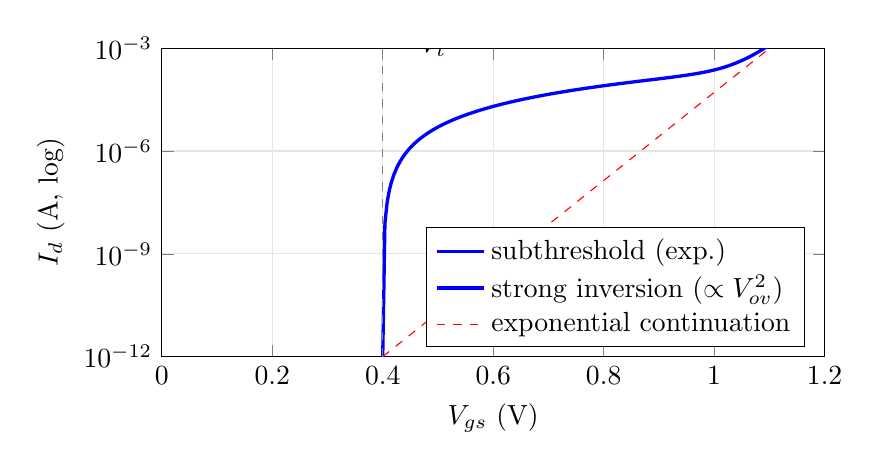
\begin{tikzpicture}
\begin{semilogyaxis}[
  width=10cm, height=5.5cm,
  xlabel={$V_{gs}$ (V)}, ylabel={$I_d$ (A, log)},
  ymin=1e-12, ymax=1e-3,
  xmin=0, xmax=1.2,
  legend pos=south east, legend cell align=left,
  grid=both, grid style={gray!20}
]
\addplot[blue, very thick, samples=200, domain=0:0.4] {1e-12 * exp((x-0.4)/0.026/1.3)};
\addlegendentry{subthreshold (exp.)}
\addplot[blue, very thick, samples=200, domain=0.4:1.2] {0.5*(x-0.4)^2 * 1e-3 + 1e-12*exp((x-0.4)/0.026/1.3)};
\addlegendentry{strong inversion ($\propto V_{ov}^2$)}
\addplot[red, dashed, samples=200, domain=0.4:1.2] {1e-12 * exp((x-0.4)/0.026/1.3)};
\addlegendentry{exponential continuation}
\draw[gray, dashed] (axis cs:0.4,1e-12) -- (axis cs:0.4,1e-3);
\node at (axis cs:0.45,3e-4) [above right] {$V_t$};
\end{semilogyaxis}
\end{tikzpicture}
\\
{\small Figure 8: $I_d$ vs $V_{gs}$ on a semilog scale. Below $V_t$ the current decays exponentially with slope $S \approx 80\,\text{mV/decade}$. ``Off'' isn't off; it's just exponentially smaller.}
\end{center}

\begin{pdnote}
With ten billion transistors at $V_t \approx 0.3\,\text{V}$, subthreshold leakage dominates static power in modern designs. Multi-$V_t$ libraries, power gating (MTCMOS), and reverse body bias are the standard PD weapons against it. The subthreshold slope $S$ is a fundamental physical limit; the search for sub-60 mV/decade devices (tunnel FETs, negative-capacitance FETs) is one of the big research themes of post-CMOS.
\end{pdnote}

\subsection{Drain-induced barrier lowering (DIBL)}

In short-channel devices, the drain voltage itself reaches into the channel and effectively \emph{lowers} the threshold:
\begin{equation}
V_t \;\approx\; V_{t0} \;-\; \eta\,V_{ds}
\end{equation}

The drain ``steals'' some of the gate's control. DIBL is one of the principal reasons FinFETs displaced planar MOSFETs near 22 nm. Wrapping the gate around the channel on three sides (FinFET) or four sides (gate-all-around) restores the electrostatic control that planar devices lose at short channels.

\begin{hook}
Picture the gate as a parent trying to control a child (the channel). In long-channel devices, the parent is right next to the child. In short-channel devices, the drain (an annoying neighbor) is also close to the child and starts giving conflicting instructions. DIBL is the channel listening to the drain instead of the gate. FinFET is the parent picking the kid up and surrounding them.
\end{hook}

\subsection{Body effect (preview)}

Already mentioned: when the source isn't at body potential ($V_{sb} \neq 0$), $V_t$ shifts. In stacked logic and SRAM bitcells this matters a lot. Full deep dive in Part II.

\subsection{Process Voltage Temperature (PVT) variation}

$V_t$ varies wafer to wafer (process corners: TT, FF, SS, FS, SF), with supply voltage (IR drop), and with temperature. \textbf{Random dopant fluctuation} adds device-to-device $V_t$ mismatch, which is especially painful for SRAM bitcells (smallest devices in the chip).

Every signoff in PD is performed across multiple PVT corners precisely because $V_t$ is not a constant.

\subsection{Leakage path checklist}

A modern transistor leaks through at least four mechanisms.
\begin{enumerate}
\item \textbf{Subthreshold leakage} (drain to source with the gate ``off''). Dominant.
\item \textbf{Gate leakage} (tunneling through the thin oxide). Cured by high-$\kappa$.
\item \textbf{Junction leakage} (reverse-biased S/B and D/B p-n junctions).
\item \textbf{Gate-induced drain leakage (GIDL)} at high $V_{dg}$. Usually small but real.
\end{enumerate}

\begin{checkpoint}
The ideal long-channel model is a useful approximation. Real chips are dominated by subthreshold leakage and short-channel effects (DIBL especially). The fixes (multi-$V_t$, FinFET, high-$\kappa$, power gating) are all responses to specific failures of the ideal model. Knowing which failure each fix targets makes you sound like you know what you're talking about.
\end{checkpoint}

\section{Why a PD Engineer at Arm Cares}

You're not going to solve Poisson's equation at the silicon surface as a PD intern. But you will:

\begin{itemize}
\item \textbf{Pick cells from a multi-$V_t$ library.} HVT for low leakage, LVT for speed. Doing this intelligently requires knowing what $V_t$ physically is.
\item \textbf{Read timing reports across PVT corners.} Slow corner is set by slow process, low voltage, worst-case temperature. All three slide $V_t$.
\item \textbf{Reason about why some cells are weak.} Stacked transistors are weak because of body effect. Long-channel devices are weak because of mobility and area. Both come from the MOS capacitor model.
\item \textbf{Manage leakage.} Always-on cells leak continuously. Power-gated regions need isolation cells. Multi-$V_t$ optimization, body biasing, and power gating are real PD knobs.
\item \textbf{Talk credibly about FinFETs and GAAFETs in interviews.} You can frame the entire FinFET justification in MOS-capacitor language: planar gate control breaks down at short channels, the fix is more electrostatic enclosure.
\end{itemize}

\begin{pdnote}
The shortcut to credibility in PD interviews is being able to tie every cell-library knob (HVT/SVT/LVT, multi-channel-length, multi-$V_{dd}$, power-gating) back to a specific physical effect in the MOSFET. Most candidates can recite ``HVT is lower leakage.'' Fewer can say ``HVT has higher $V_t$ because of heavier channel doping, which makes the depletion-charge term bigger, which suppresses subthreshold leakage exponentially.''
\end{pdnote}

\section{Common Mistakes}

\begin{enumerate}
\item \textbf{Treating ``off'' as ``no current.''} Subthreshold current is real and exponential in $V_{gs}$. A transistor below $V_t$ leaks, just exponentially less than above $V_t$.
\item \textbf{Treating $V_t$ as fixed.} $V_t$ depends on body bias, drain voltage (DIBL), channel length, temperature, and process corner. It's a characteristic, not a constant.
\item \textbf{Confusing ``depletion mode'' with depletion-mode transistors.} ``Depletion mode'' in our context means a surface state. A \emph{depletion-mode MOSFET} is a separate, specialized device that conducts at $V_{gs} = 0$ thanks to a built-in channel. Different concept, same vocabulary.
\item \textbf{Memorizing $Q_{inv} = C_{ox}(V_{gs}-V_t)$ without knowing it's an approximation.} It's the charge-sheet, strong-inversion approximation. The real subthreshold transition is gradual.
\item \textbf{Sign confusion on PMOS.} PMOS has a negative $V_t$. Either write equations with $|V_{tp}|$ or be explicit about sign conventions throughout.
\item \textbf{Ignoring the body terminal.} Beginner schematics often omit the body because it's tied to a rail by default. In stacked logic, SOI, and triple-well processes, the body absolutely matters.
\item \textbf{Treating the gate as electrically connected to the channel.} It's not. There's an insulator in between. The gate controls the channel \emph{capacitively}. That's exactly why gate leakage is a problem at thin oxides: classically it shouldn't exist at all.
\end{enumerate}

\section{Interview-Ready 90-Second Answer}

\begin{quote}\itshape
A MOSFET is fundamentally a MOS capacitor with two contacts. Applying a voltage to the gate modulates the charge in the silicon surface underneath. For an NMOS with a negative gate, you accumulate holes, and the device is off. Make the gate slightly positive and you push the holes away, creating a depletion region of ionized acceptors; still off. Push the gate above threshold and you invert the surface; mobile electrons appear and connect source to drain, and the device is on. The inversion charge above threshold is $C_{ox}(V_{gs}-V_t)$, which sets the drain current and the on-resistance. PMOS works by symmetry with the signs flipped. In real devices we also care about subthreshold leakage, body effect, DIBL, and PVT variation; all are second-order effects layered on top of the same MOS-capacitor physics.
\end{quote}

That's about ninety seconds spoken aloud. Practice it. Out loud. To a mirror. Until it's muscle memory.

\section{Practice Problems for Part I}

\textbf{Q1 (conceptual).} Explain in two sentences why the MOS capacitance drops in depletion but returns to $C_{ox}$ in strong inversion at low frequency.

\textbf{Q2 (numerical).} An NMOS has $V_{t0} = 0.4\,\text{V}$, $\gamma = 0.3\sqrt{V}$, $2\phi_F = 0.6\,\text{V}$. In a NAND2, the upper NMOS sees $V_{sb} = 0.3\,\text{V}$. Compute the effective $V_t$.

\textbf{Q3 (PD-flavored).} A timing path fails by $50\,\text{ps}$. The path has 6 SVT cells. What cells would you swap to LVT, and what is the leakage tradeoff in physical terms?

\textbf{Q4 (explain-back).} In three sentences, explain (a) what threshold voltage is, (b) why it depends on doping, and (c) why this matters for HVT/SVT/LVT cell libraries.

\textbf{Q5 (stretch).} Sketch a C to V curve at low frequency. Label $V_{FB}$, $V_t$, accumulation, depletion, inversion. Redraw the high-frequency version and explain what's different.

\vspace{0.5em}\hrule\vspace{0.5em}
\noindent\textit{Companion video for Part I:} VLSI Academy, ``PD Lec 3: CMOS Basics part 2'' (\url{https://youtu.be/WPBkjAmjqzw}).

% =========================================================
\part*{Part II: Second-Order Effects (Body Effect and CLM)}
\addcontentsline{toc}{part}{Part II: Second-Order Effects}
\textit{A first-principles companion to VLSI Academy PD Lec 4.}

\section{Why We Need a Part II}

\begin{tldr}
\begin{itemize}[leftmargin=*]
\item Part I assumed two things that aren't quite true: that the body terminal sits at the same potential as the source, and that saturation current is perfectly flat in $V_{ds}$.
\item Body effect: $V_t$ shifts when the source isn't at body potential. This is why stacked NMOS devices in NAND gates are weaker than singles.
\item Channel length modulation: $I_d$ keeps creeping up with $V_{ds}$ even in saturation, because the effective channel length shrinks. This sets the analog gain of every MOSFET stage you'll ever design.
\item ``Second-order'' doesn't mean ``small.'' These can shift $V_t$ by 100 mV and set $r_o$ over orders of magnitude.
\end{itemize}
\end{tldr}

Part I built the MOSFET from the MOS capacitor up. The picture was idealized in two important ways.

\begin{enumerate}
\item We assumed the body terminal sits at the same potential as the source, so $V_{sb} = 0$. Threshold voltage was a fixed material property.
\item We wrote the saturation drain current as a clean function of $V_{ov}^2$ that does not depend on $V_{ds}$ at all.
\end{enumerate}

Both assumptions break down in real silicon. Part II treats the two corrections you encounter first, and most often, in physical design work.

\begin{keyidea}
A ``second-order effect'' does not mean ``small.'' It means ``not in the first-order model.'' Body effect can shift $V_t$ by 100 mV or more in stacked logic. Channel length modulation sets the entire output resistance of every MOSFET in your analog datapath. Treat them as first-class citizens.
\end{keyidea}

\section{Body Effect}

\begin{tldr}
\begin{itemize}[leftmargin=*]
\item In any chip, the body (substrate) is a single big chunk of silicon shared by every NMOS. You cannot give each transistor its own private body voltage.
\item Source nodes can sit at any voltage between the rails. So $V_{sb}$ varies device by device.
\item When $V_{sb} > 0$, the depletion region under the gate widens. The gate has to support more depletion charge. $V_t$ rises.
\item Always ground the body (or tie n-well to $V_{dd}$). The body-effect formula assumes a stable reference; layout enforces it with body ties.
\end{itemize}
\end{tldr}

\subsection{The setup: why this even comes up}

In Part I we wrote the threshold voltage assuming the source and body sat at the same electrical potential. In a real chip, the body is shared. The source is per-device.

When you stack transistors (NAND, NOR, pass-transistor logic, SRAM access transistors), the source of the upper device is held above ground by whatever is below it. That means $V_{sb} > 0$ for the upper device, even though the lower device has $V_{sb} = 0$.

\subsection{The physical mechanism}

Reverse-bias the body relative to the source ($V_{sb} > 0$ for an NMOS). From the surface's point of view, you have just added \emph{more} band bending to overcome before you can reach strong inversion.

\begin{enumerate}
\item More band bending means a wider depletion region.
\item Wider depletion region means more fixed acceptor ions exposed.
\item More fixed acceptor ions means more depletion charge the gate must support.
\item More depletion charge to support means a higher gate voltage is needed to reach inversion.
\item Higher gate voltage to reach inversion means a higher $V_t$.
\end{enumerate}

\begin{keyidea}
Reverse-biasing the body widens the depletion region. A wider depletion region holds more fixed charge. The gate has to overcome more charge to invert the surface. Therefore $V_t$ rises with $V_{sb}$.
\end{keyidea}

\begin{hook}
Picture the gate as you, trying to push a stack of books off a table. Normally there are 5 books on the table. You can push them off with a moderate shove (low $V_t$). Body effect is somebody secretly adding 3 more books to the stack while you're not looking. Now you need a stronger shove (higher $V_t$) to get the same result.
\end{hook}

\subsection{The formula}

\begin{equation}
\boxed{V_t \;=\; V_{t0} \;+\; \gamma\Big(\sqrt{2\phi_F + V_{sb}} \;-\; \sqrt{2\phi_F}\Big)}
\end{equation}
where
\begin{equation}
\gamma \;=\; \frac{\sqrt{2q\varepsilon_{si}N_A}}{C_{ox}}
\end{equation}
is the \textbf{body-effect coefficient}, with units of $\sqrt{V}$.

\begin{center}
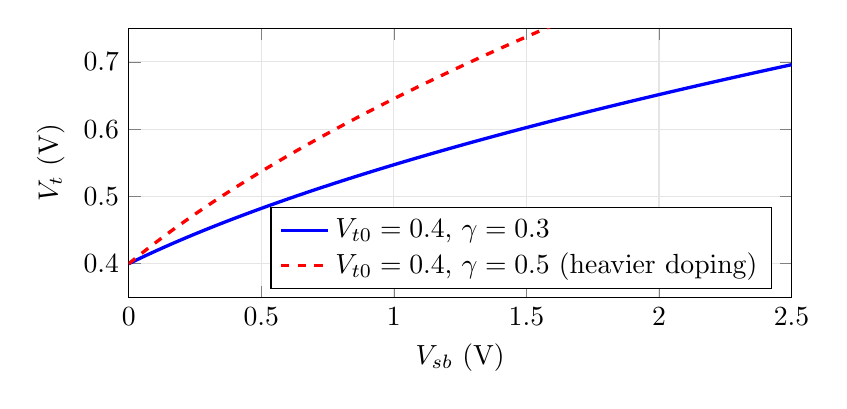
\begin{tikzpicture}
\begin{axis}[
  width=10cm, height=5cm,
  xlabel={$V_{sb}$ (V)}, ylabel={$V_t$ (V)},
  xmin=0, xmax=2.5, ymin=0.35, ymax=0.75,
  legend pos=south east, legend cell align=left,
  domain=0:2.5, samples=80, grid=major, grid style={gray!20}
]
\addplot[blue, very thick] {0.4 + 0.3*(sqrt(0.6+x) - sqrt(0.6))};
\addlegendentry{$V_{t0}=0.4$, $\gamma=0.3$}
\addplot[red, dashed, very thick] {0.4 + 0.5*(sqrt(0.6+x) - sqrt(0.6))};
\addlegendentry{$V_{t0}=0.4$, $\gamma=0.5$ (heavier doping)}
\end{axis}
\end{tikzpicture}
\\
{\small Figure 9: $V_t$ vs $V_{sb}$. Higher channel doping (larger $\gamma$) gives a stronger body effect. Slope is steepest near $V_{sb}=0$ and flattens as $V_{sb}$ grows.}
\end{center}

\subsection{Worked example: how bad is it?}

\textbf{Setup.} NMOS with $V_{t0} = 0.4\,\text{V}$, $\gamma = 0.3\sqrt{V}$, $2\phi_F = 0.6\,\text{V}$. In a NAND2, the upper NMOS sees its source held at roughly $0.3\,\text{V}$ above ground. So $V_{sb} = 0.3\,\text{V}$.

\textbf{Compute the $V_t$ shift.}
\[
\Delta V_t = 0.3 \cdot \big(\sqrt{0.6 + 0.3} - \sqrt{0.6}\big) = 0.3 \cdot (0.9487 - 0.7746) = 0.3 \cdot 0.1741 \approx 0.052\,\text{V}
\]
\[
V_t \;\approx\; 0.452\,\text{V}
\]

\textbf{What this means.} The upper NMOS effectively has a 13\% higher $V_t$ than the lower one. Its $V_{ov} = V_{gs} - V_t$ is smaller for the same $V_{gs}$. Since $I_d \propto V_{ov}^2$ in saturation, the upper device's drive strength drops by roughly 25\% for typical supplies. That's why the upper NMOS in a NAND stack feels ``weak.''

\begin{gut}
If the stack went three high (NAND3) and the topmost device saw $V_{sb} = 0.6\,\text{V}$, would the shift be bigger or smaller than $2\times 0.052$? (Answer: bigger, but the slope flattens, so not $2\times$. Plug in: $\Delta V_t \approx 0.3 \cdot (\sqrt{1.2} - \sqrt{0.6}) = 0.3 \cdot 0.3210 \approx 0.096\,\text{V}$.)
\end{gut}

\subsection{The lecturer's emphasis: ground the body to kill noise}

The PD Lec 4 video spends most of its body-effect minutes on a related but distinct point: \textbf{you should hard-ground the substrate so noise spikes on the body do not modulate $V_t$.}

The reasoning is straightforward. The $V_t$ formula tells you that any change in $V_{sb}$ changes $V_t$. If the body is allowed to float or is loosely connected, capacitive coupling from neighboring switching nodes will dump charge onto it, and your transistor's threshold will wobble at exactly the worst moments (when its neighbors are switching).

Foundries enforce this with explicit \textbf{body ties}: heavily doped p+ contacts to the p-substrate placed at regular intervals across the layout, all hard-wired to ground. PD layout rules typically specify a maximum distance between any device and its nearest body tie, exactly so that no part of the substrate can drift far from ground potential.

\begin{pdnote}
When you see a DRC error about ``well tap distance,'' you are bumping into the body-effect noise-immunity rule. The rule exists because the entire body-effect formula assumes the body is at a known, stable potential. The minute that assumption breaks, your timing characterization is wrong.
\end{pdnote}

\begin{hook}
Body ties are like grounding straps on a static-sensitive workbench. You don't notice them when they're working. The moment one comes loose, sparks fly and circuits get fried.
\end{hook}

\subsection{Common mistakes}

\begin{enumerate}
\item \textbf{Assuming $V_{sb}$ is always zero.} Zero only for the bottommost NMOS in a stack (or the topmost PMOS). Every other device sees some body effect.
\item \textbf{Reading the formula and concluding body effect is small.} For a single device at $V_{sb} = 0.3\,\text{V}$ it's a $50\,\text{mV}$ shift. For a 4-high pass-transistor stack, the topmost device can see hundreds of mV. Destroys timing and noise margin.
\item \textbf{Ignoring body effect in PMOS.} It works identically with signs flipped: n-well tied to $V_{dd}$, any PMOS with source below $V_{dd}$ sees $|V_{tp}|$ grow.
\item \textbf{Confusing body effect with body biasing.} Body biasing is the designer deliberately offsetting body voltage to tune $V_t$ for power-performance trade-offs. Body effect is the underlying physics that body biasing exploits.
\end{enumerate}

\begin{checkpoint}
Body effect rule of thumb: stacked devices are weaker because their sources sit above ground (NMOS) or below $V_{dd}$ (PMOS), reverse-biasing their bodies and raising $|V_t|$. Always ground the substrate and tie the n-well to $V_{dd}$ so the formula has a stable reference. Watch the topmost device in any stack first.
\end{checkpoint}

\section{Channel Length Modulation}

\begin{tldr}
\begin{itemize}[leftmargin=*]
\item In Part I we said saturation current is flat in $V_{ds}$. Not quite. It creeps up with $V_{ds}$.
\item The reason: once $V_{ds} > V_{ov}$, the channel pinches off short of the drain. The pinch-off point moves closer to the source as $V_{ds}$ grows.
\item Effective channel length $L' = L - \Delta L$ shrinks. Since $I_d \propto 1/L$, $I_d$ rises.
\item Formula: $I_d = I_{d0}(1 + \lambda V_{ds})$. Output resistance $r_o = 1/(\lambda I_d)$.
\item This sets analog gain, and gets worse as $L$ shrinks. Long-channel devices for high gain; short-channel for speed.
\end{itemize}
\end{tldr}

\subsection{The setup: why the curves aren't flat}

Look back at the I to V family plot in Part I. In saturation, the curves look \emph{almost} flat but not quite. They have a gentle upward slope. That slope is what channel length modulation refers to.

It's the MOSFET analogue of the Early effect in BJTs. Same idea, slightly different mechanism.

\subsection{What ``pinch-off'' actually means (review)}

Recall the channel charge per unit area at a point $y$ along the channel:
\[
Q_{inv}(y) \;=\; C_{ox}\,[V_{gs} - V(y) - V_t]
\]

At the source end, $V(0) = 0$, so the channel is thickest. At the drain end, $V(L) = V_{ds}$, so the channel is thinnest.

When $V_{ds}$ reaches $V_{ov}$, the local gate-overdrive at the drain end falls to zero. The inversion charge vanishes at that point. The channel has \emph{pinched off}.

\begin{hook}
Pinch-off is like a garden hose with a kink near the nozzle. Water still flows through it (carriers still cross the pinch-off region by drift in high field), but the bottleneck is fixed. Cranking the faucet harder (raising $V_{ds}$) doesn't push much more water through, because the kink itself is the limit.
\end{hook}

\subsection{Where the second-order effect comes from}

Here's the subtlety. Pinch-off does not happen at exactly $y = L$. Once $V_{ds} > V_{ov}$, the pinch-off point moves \emph{inside} the channel, at some position $y = L' < L$. Beyond $L'$, between $L'$ and the drain, there is no inversion layer. That region is a depletion region that carriers traverse by drift in a very high electric field.

As you raise $V_{ds}$ further, the pinch-off point moves further toward the source. The effective conducting length of the channel, $L'$, shrinks. Call the shrinkage $\Delta L$, so $L' = L - \Delta L$.

Now recall that drain current in saturation is inversely proportional to $L$:
\[
I_d \;\propto\; \frac{1}{L}
\]

If the effective $L$ shrinks, $I_d$ rises. That's channel length modulation.

\begin{center}
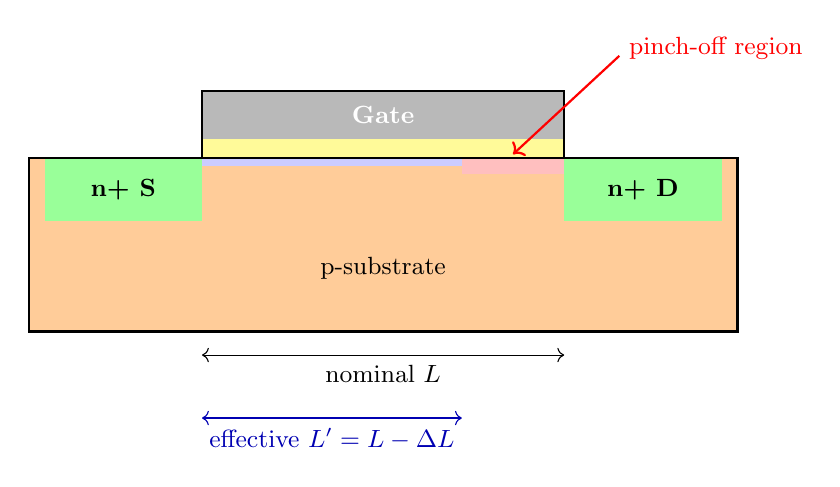
\begin{tikzpicture}[font=\small,scale=1.0]
  \fill[orange!40] (0,0) rectangle (9,2.2);
  \fill[green!40]  (0.2,1.4) rectangle (2.2,2.2);
  \fill[green!40]  (6.8,1.4) rectangle (8.8,2.2);
  \fill[blue!20]   (2.2,2.1) rectangle (5.5,2.2);
  \fill[red!25]    (5.5,2.0) rectangle (6.8,2.2);
  \fill[yellow!40] (2.2,2.2) rectangle (6.8,2.45);
  \fill[gray!55]   (2.2,2.45) rectangle (6.8,3.05);
  \draw[thick] (0,0) rectangle (9,2.2);
  \draw[thick] (2.2,2.2) rectangle (6.8,3.05);
  \node at (1.2,1.8) {\textbf{n+ S}};
  \node at (7.8,1.8) {\textbf{n+ D}};
  \node[white] at (4.5,2.75) {\textbf{Gate}};
  \node at (4.5,0.8) {\small p-substrate};
  \draw[<->] (2.2,-0.3) -- (6.8,-0.3) node[midway,below] {nominal $L$};
  \draw[<->,blue!70!black] (2.2,-1.1) -- (5.5,-1.1) node[midway,below] {\small effective $L' = L - \Delta L$};
  \draw[red,->,thick] (7.5,3.5) -- (6.15,2.25);
  \node[red,right] at (7.5,3.6) {\small pinch-off region};
\end{tikzpicture}
\\
{\small Figure 10: Channel length modulation. Once $V_{ds} > V_{ov}$, the inversion channel pinches off short of the drain. Increasing $V_{ds}$ pushes the pinch-off point further toward the source, shortening $L'$ and raising $I_d$.}
\end{center}

\subsection{The formula}

\begin{equation}
\boxed{I_d \;=\; \tfrac{1}{2}\mu_n C_{ox}\frac{W}{L}(V_{gs}-V_t)^2\,(1 + \lambda V_{ds})}
\end{equation}

The parameter $\lambda$ (units of $V^{-1}$) is the channel-length modulation coefficient. Long-channel devices have small $\lambda$ (close to zero). Short-channel devices have large $\lambda$.

The small-signal output resistance is:
\begin{equation}
\boxed{r_o \;=\; \frac{1}{\lambda I_d}}
\end{equation}

\begin{keyidea}
$r_o = 1/(\lambda I_d)$ is the single most important small-signal parameter of a MOSFET for analog design. It sets the intrinsic gain $g_m \cdot r_o$ of every common-source amplifier. Analog designers grumble about short-channel processes because $\lambda$ rises (and $r_o$ falls) as $L$ shrinks.
\end{keyidea}

\subsection{Plotting the effect}

\begin{center}
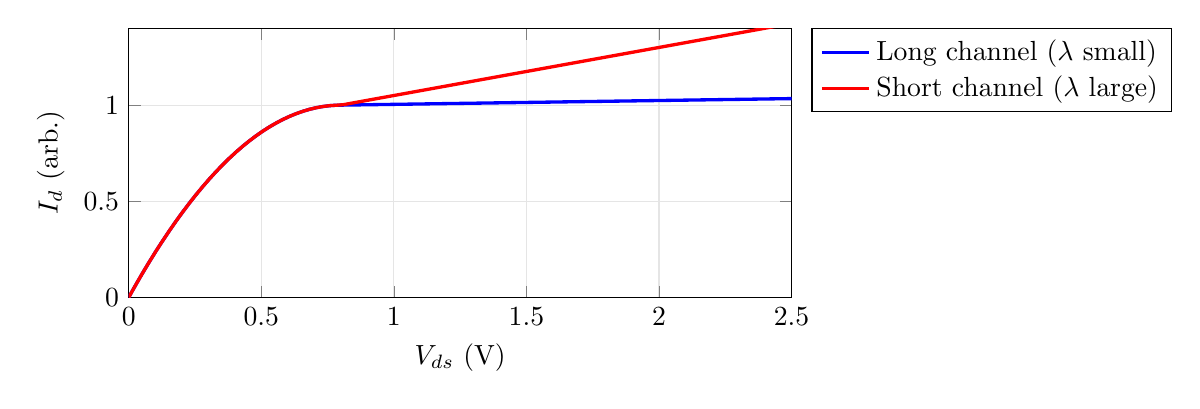
\begin{tikzpicture}
\begin{axis}[
  width=10cm, height=5cm,
  xlabel={$V_{ds}$ (V)}, ylabel={$I_d$ (arb.)},
  xmin=0, xmax=2.5, ymin=0, ymax=1.4,
  legend pos=outer north east, legend cell align=left,
  domain=0:2.5, samples=80, grid=major, grid style={gray!20}
]
\addplot[blue, very thick, samples=100] {(x<0.8) * (0.8*x - 0.5*x*x) * 1.0/0.32 + (x>=0.8) * 1.0 * (1 + 0.02*(x-0.8))};
\addlegendentry{Long channel ($\lambda$ small)}
\addplot[red, very thick, samples=100] {(x<0.8) * (0.8*x - 0.5*x*x) * 1.0/0.32 + (x>=0.8) * 1.0 * (1 + 0.25*(x-0.8))};
\addlegendentry{Short channel ($\lambda$ large)}
\end{axis}
\end{tikzpicture}
\\
{\small Figure 11: Channel length modulation. Long-channel devices look ideal (flat $I_d$ in saturation). Short-channel devices have a noticeable upward slope, equivalent to a finite $r_o$. Extrapolating the saturation line backward to $I_d = 0$ defines $V_A = 1/\lambda$, analogous to the BJT Early voltage.}
\end{center}

\subsection{Worked example: compute $r_o$ and intrinsic gain}

\textbf{Setup.} Short-channel NMOS in saturation. $\mu_n C_{ox} = 100\,\mu\text{A}/\text{V}^2$, $W/L = 2$, $V_{ov} = 0.4\,\text{V}$, $\lambda = 0.1\,V^{-1}$, $V_{ds} = 1\,\text{V}$.

\textbf{Compute $I_d$.}
\[
I_{d0} = \tfrac{1}{2}\cdot 100\,\mu\text{A}/\text{V}^2 \cdot 2 \cdot (0.4)^2 = 16\,\mu\text{A}
\]
\[
I_d = 16\,\mu\text{A}\cdot(1 + 0.1\cdot 1) = 17.6\,\mu\text{A}
\]
A 10\% current bump from channel length modulation alone.

\textbf{Compute output resistance.}
\[
r_o = \frac{1}{\lambda I_d} = \frac{1}{0.1\cdot 17.6\,\mu\text{A}} \approx 568\,\text{k}\Omega
\]

\textbf{Compute intrinsic gain.} Transconductance is $g_m \approx 2I_d / V_{ov} = 88\,\mu\text{A/V}$. So:
\[
A_v = g_m\, r_o = 88\,\mu\text{A/V} \cdot 568\,\text{k}\Omega \approx 50
\]

That's the gain of a single common-source stage with an ideal current source load. Halve $\lambda$ and you double the gain. That's why analog designers fight for long-channel devices.

\subsection{Why this matters in PD work}

\begin{itemize}
\item \textbf{Short-channel effects.} As $L$ shrinks, $\lambda$ rises. Drive currents in the latest nodes don't scale as cleanly as Dennard scaling once predicted.
\item \textbf{DIBL.} CLM's electrostatic cousin. At very short channels, the drain field reaches the source and lowers $V_t$ as $V_{ds}$ rises. The leakage path you live in fear of ($I_{\text{off}}$) is set partly by DIBL.
\item \textbf{Library characterization.} Standard cell libraries are characterized across $V_{ds}$ so $(1 + \lambda V_{ds})$ is captured in timing arcs.
\item \textbf{Long-channel for stability.} In bias generation (PMU references, bandgaps), long-channel devices are used deliberately to minimize $\lambda$ and maximize $r_o$.
\end{itemize}

\subsection{Common mistakes}

\begin{enumerate}
\item \textbf{Treating saturation as perfectly flat.} It isn't. Always include $(1 + \lambda V_{ds})$ for any small-signal or output-resistance calculation.
\item \textbf{Confusing channel length modulation with DIBL.} CLM modulates the \emph{effective} length while $V_t$ stays put. DIBL modulates $V_t$ itself. They look similar in measured $I_d$ to $V_{ds}$ curves but have different physical origins.
\item \textbf{Assuming $\lambda$ is a single number.} $\lambda$ depends on $L$, $V_{ds}$, and bias point. SPICE BSIM models capture this; hand calculations use a representative average.
\item \textbf{Forgetting that $r_o$ is current-dependent.} A device at 1 mA has $1000\times$ smaller $r_o$ than the same device at 1 $\mu$A.
\end{enumerate}

\begin{checkpoint}
Channel length modulation is the simple geometric story: pinch-off moves toward the source as $V_{ds}$ rises, shrinking effective $L$ and lifting $I_d$. The price is finite output resistance $r_o = 1/(\lambda I_d)$, which sets analog gain and ties directly to short-channel behavior in modern nodes.
\end{checkpoint}

\section{How Body Effect and CLM Connect to Real PD Work}

These two effects collectively explain a long list of behaviors you will see during physical implementation work.

\begin{itemize}
\item \textbf{Stack-of-N is not $N\times$ as bad.} You might expect 4 NMOS in series to have $4\times$ the on-resistance of a single device. It's worse. Each successive device upward sees a larger $V_{sb}$, larger $V_t$, smaller $V_{ov}$, non-linearly larger $R_{on}$. Logic synthesis accounts for this when sizing stacks.
\item \textbf{Setup and hold across PVT.} Body effect interacts with temperature ($\phi_F$ is temperature-dependent) and with supply IR drop. The slow corner is doubly hurt: lower $V_{dd}$ means more devices feel more body effect.
\item \textbf{Analog gain falls with each node shrink.} CLM gets worse as $L$ shrinks. A 28 nm long-channel device might give single-stage gain of 100; a 7 nm minimum-length device might give 5. Analog designers cascode to recover.
\item \textbf{Substrate noise and ground bounce.} Both effects assume body is a stable reference. When the substrate bounces from heavy switching, $V_{sb}$ wobbles, $V_t$ wobbles, timing breaks. Cure: dense body ties and decoupling.
\end{itemize}

\section{Self-Check Questions for Part II}

\textbf{Q1 (body effect, conceptual).} Explain in three sentences why widening the depletion region under the gate raises $V_t$. Use the words ``fixed acceptor charge'' and ``gate must support.''

\textbf{Q2 (body effect, numerical).} NMOS with $V_{t0} = 0.35\,\text{V}$, $\gamma = 0.45\sqrt{V}$, $2\phi_F = 0.7\,\text{V}$. Topmost in a 3-high pass stack with $V_{sb} = 0.6\,\text{V}$. Compute effective $V_t$. By what factor is its $I_d$ reduced relative to the bottom device, assuming both see $V_{gs} = 1.0\,\text{V}$?

\textbf{Q3 (CLM, conceptual).} Explain why pinch-off doesn't happen exactly at $y = L$ when $V_{ds} > V_{ov}$. Sketch.

\textbf{Q4 (CLM, numerical).} MOSFET with $g_m = 200\,\mu\text{A/V}$, $I_d = 50\,\mu\text{A}$, $\lambda = 0.04\,V^{-1}$. Compute $r_o$ and single-stage intrinsic gain.

\textbf{Q5 (synthesis).} A PD reviewer flags that the topmost NMOS in a 4-input NOR-equivalent pull-down stack should be upsized. Explain why in two sentences, citing body effect.

\textbf{Q6 (synthesis).} You're sizing a long-channel current mirror in a bandgap reference. Why do analog designers reach for $L = 5\times$ minimum or more here?

\vspace{0.5em}\hrule\vspace{0.5em}
\noindent\textit{Companion video for Part II:} VLSI Academy, ``PD Lec 4: CMOS Basics part 3'' (\url{https://youtu.be/Ni7TRr2oXzE}).

% =========================================================
\part*{Part III: Short-Channel Effects and Modern Devices}
\addcontentsline{toc}{part}{Part III: Short-Channel Effects and Modern Devices}
\textit{Where the long-channel model breaks, and what foundries did about it.}

\section{Why a Part III}

\begin{tldr}
\begin{itemize}[leftmargin=*]
\item The long-channel model assumed the gate had absolute control of the channel and that carriers obeyed a simple mobility law. At sub-100 nm $L$, both assumptions break.
\item Velocity saturation: carriers stop accelerating in high field. Drain current scales linearly with $V_{ov}$, not quadratically.
\item DIBL and punch-through: the drain field reaches the source and steals control from the gate. Threshold drops with $V_{ds}$.
\item FinFETs and gate-all-around (GAAFETs) restore electrostatic control by wrapping the gate around the channel.
\item Variability (random dopant fluctuation, line-edge roughness) becomes a first-class design concern below 28 nm.
\end{itemize}
\end{tldr}

The MOSFET model in Parts I and II is the textbook long-channel device. Useful for intuition. Increasingly inaccurate for any real silicon you will work on at Arm. Part III is a curated tour of the second-order effects you will see called out in datasheets, timing reports, and library release notes.

\section{Velocity Saturation (the speed limit)}

\begin{tldr}
\begin{itemize}[leftmargin=*]
\item At low fields, carrier drift velocity is proportional to field: $v = \mu E$.
\item At fields above $\approx 10^4\,\text{V/cm}$ in silicon, scattering dominates and $v$ saturates at $v_{sat} \approx 1 \times 10^7\,\text{cm/s}$ for electrons.
\item In short-channel MOSFETs, the lateral field along the channel hits $v_{sat}$ even at modest $V_{ds}$.
\item Consequence: $I_d$ becomes linear, not quadratic, in $V_{ov}$. The $V_{ov}^2$ formula overstates drive in modern nodes.
\end{itemize}
\end{tldr}

\subsection{Where the simple drift law breaks}

In Part I we wrote drain current as $I_d = Q_{inv}\cdot v$. We then quietly assumed $v = \mu E$, with mobility $\mu$ a constant. That holds at low fields. At high fields, $v$ stops growing.

The lateral field along the channel is roughly $V_{ds}/L$. For $V_{ds} = 1\,\text{V}$ and $L = 30\,\text{nm}$, that's $E \approx 3.3\times 10^5\,\text{V/cm}$, well above the saturation threshold. Electrons in such a field move at a hard cap of $v_{sat} \approx 10^7\,\text{cm/s}$.

\subsection{The velocity-saturated drain current}

In the fully velocity-saturated limit:
\begin{equation}
I_d \;\approx\; W\,C_{ox}\,(V_{gs} - V_t)\,v_{sat}
\end{equation}

Notice: \textbf{$I_d$ is linear in $V_{ov}$, not quadratic.} Also, $L$ drops out of the equation entirely. That has a big consequence: shrinking $L$ no longer linearly buys you current. Dennard scaling stalls.

\begin{keyidea}
Velocity saturation turns the square-law transistor into a linear one. The $V_{ov}^2$ formula overstates drive current in modern nodes. Treat it as a first-order ceiling and de-rate.
\end{keyidea}

\begin{hook}
Carriers in high field are like cars in heavy traffic. At low density (low field) every driver picks their own speed and you can go faster by stepping on the gas (higher $E$, higher $v$). At high density (high field), everyone is bumper-to-bumper at the same speed regardless of how hard you press the pedal. The pedal stops working past a point. That's $v_{sat}$.
\end{hook}

\subsection{Worked example: when does velocity saturation matter?}

\textbf{Setup.} NMOS at the $7\,\text{nm}$ node. $L_{\text{eff}} \approx 20\,\text{nm}$. Critical field for velocity saturation $E_c \approx 4\times 10^4\,\text{V/cm}$. Find the $V_{ds}$ at which the average lateral field exceeds $E_c$.

\[
V_{ds} = E_c \cdot L_{\text{eff}} = 4\times 10^4 \cdot 20\times 10^{-7} = 0.08\,\text{V}
\]

A measly $80\,\text{mV}$ across the channel and you're already in velocity saturation. At any realistic supply ($\geq 0.7\,\text{V}$), the device lives in the saturated-velocity regime end-to-end.

\begin{pitfall}
Hand calculations using the textbook $I_d = \tfrac{1}{2}\mu C_{ox}\frac{W}{L}V_{ov}^2$ formula at advanced nodes will over-predict drive current by $2\times$ to $3\times$. Use it for ranking and sanity, not for sign-off. SPICE BSIM models capture velocity saturation correctly.
\end{pitfall}

\section{DIBL Deep Dive and Punch-Through}

\begin{tldr}
\begin{itemize}[leftmargin=*]
\item DIBL: the drain depletion region reaches into the channel, lowering the energy barrier source-to-channel, lowering $V_t$ effectively.
\item Punch-through: the drain depletion region touches the source depletion region. Subthreshold current explodes regardless of gate.
\item Both are pure short-channel effects. Long-channel devices don't see them.
\item Cures: halo implants (raise local doping near S/D), thinner oxide (more gate control), and ultimately FinFET / GAAFET geometry.
\end{itemize}
\end{tldr}

\subsection{The barrier picture}

Think of source-to-channel as an energy barrier (the n+ source is full of electrons; they have to climb a barrier set by the channel doping and the gate voltage to enter the channel). In a long-channel device, the gate sets the height of that barrier. The drain is far away and irrelevant to the barrier.

In a short-channel device, the drain depletion region extends a noticeable distance into the channel. Its built-in field, plus any $V_{ds}$, reaches across and \emph{pulls down} the barrier near the drain edge.

The result: electrons climb a smaller barrier. Effective $V_t$ drops as $V_{ds}$ rises:
\begin{equation}
V_t \;\approx\; V_{t0} \;-\; \eta\, V_{ds}, \qquad \eta \approx 10 \text{ to } 100\,\text{mV/V}
\end{equation}

\subsection{Worked DIBL example}

\textbf{Setup.} Short-channel NMOS with $\eta = 50\,\text{mV/V}$, $V_{t0} = 0.35\,\text{V}$. Compute effective $V_t$ at $V_{ds} = 0.05\,\text{V}$ (linear measurement) and $V_{ds} = 0.9\,\text{V}$ (saturation operating point).

\[
V_t(0.05) = 0.35 - 0.050 \cdot 0.05 = 0.3475\,\text{V}
\]
\[
V_t(0.9) = 0.35 - 0.050 \cdot 0.9 = 0.305\,\text{V}
\]

A $45\,\text{mV}$ threshold shift. In subthreshold (slope $\sim 80\,\text{mV/decade}$) that's roughly $10^{45/80} \approx 3.6\times$ more leakage current at the operating $V_{ds}$ vs the linear measurement. DIBL is a major contributor to $I_{\text{off}}$ in modern leaky devices.

\subsection{Punch-through (the catastrophic version)}

Crank $V_{ds}$ even higher in a short-channel device. The drain depletion region eventually touches the source depletion region. At that point, the channel barrier is essentially gone. Subthreshold current spikes by orders of magnitude.

Foundries prevent punch-through with \textbf{halo (or pocket) implants}: localized higher-doping pockets near the source and drain that keep depletion widths short. You will never tune this. But you will see it called out as a process feature in the PDK release notes.

\begin{pdnote}
DIBL is why you see leakage characterized across $V_{dd}$ in the timing release. Higher $V_{dd}$ doesn't just raise dynamic power; it raises static power exponentially via DIBL lowering $V_t$. PD leakage recovery scripts know this. They preferentially fix high-$V_{dd}$ paths first.
\end{pdnote}

\section{FinFETs and Gate-All-Around (the geometric fix)}

\begin{tldr}
\begin{itemize}[leftmargin=*]
\item Planar MOSFETs control the channel from one side (the top). Below 22 nm, that's not enough; DIBL and subthreshold leakage get out of hand.
\item FinFETs: stand the channel up as a thin vertical ``fin'' and wrap the gate around three sides. More gate control, less drain leakage.
\item GAAFETs (also called nanosheet, nanowire): wrap the gate around all four sides of a stack of horizontal silicon ``sheets.'' Even more control, used at 3 nm and below.
\item Layout consequence: device widths quantize. A FinFET has integer number of fins; you can't draw arbitrary $W$.
\end{itemize}
\end{tldr}

\subsection{The electrostatic argument}

A MOSFET's short-channel behavior is set by how well the gate ``dominates'' the channel against the drain. The figure of merit is the natural length:
\begin{equation}
\lambda_n \;\sim\; \sqrt{\frac{\varepsilon_{si}}{\varepsilon_{ox}}\, t_{ox}\, t_{si}}
\end{equation}
where $t_{si}$ is the effective silicon body thickness. Short-channel effects are tolerable when $L \gg \lambda_n$.

To shrink $L$, you must shrink $\lambda_n$. Two knobs: thinner $t_{ox}$ (limited by gate leakage) and thinner $t_{si}$ (the geometric body).

\textbf{FinFET} makes $t_{si}$ small by literally making the silicon body a thin vertical fin (typically $5$ to $8\,\text{nm}$ thick). The gate wraps over the top and both sides.

\textbf{GAAFET} (nanosheet) makes $t_{si}$ even smaller by stacking thin horizontal silicon sheets ($5\,\text{nm}$ thick or less) with the gate fully surrounding each sheet.

\begin{center}
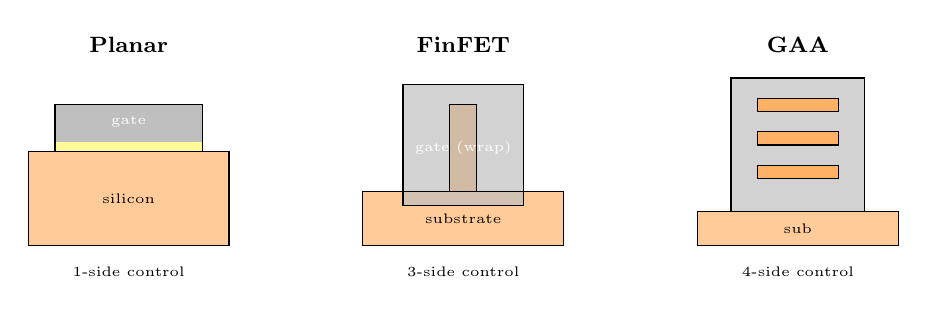
\begin{tikzpicture}[font=\footnotesize, scale=0.85]
  % Planar
  \begin{scope}
    \node at (1.5,3) {\textbf{Planar}};
    \fill[orange!40] (0,0) rectangle (3,1.4);
    \fill[yellow!40] (0.4,1.4) rectangle (2.6,1.55);
    \fill[gray!50]   (0.4,1.55) rectangle (2.6,2.1);
    \draw (0,0) rectangle (3,1.4);
    \draw (0.4,1.4) rectangle (2.6,2.1);
    \node at (1.5,0.7) {\tiny silicon};
    \node[white] at (1.5,1.85) {\tiny gate};
    \node at (1.5,-0.4) {\tiny 1-side control};
  \end{scope}
  % FinFET
  \begin{scope}[xshift=5cm]
    \node at (1.5,3) {\textbf{FinFET}};
    \fill[orange!40] (0,0) rectangle (3,0.8);
    \fill[orange!60] (1.3,0.8) rectangle (1.7,2.1);
    \fill[gray!50, opacity=0.7] (0.6,0.6) rectangle (2.4,2.4);
    \draw (0,0) rectangle (3,0.8);
    \draw (1.3,0.8) rectangle (1.7,2.1);
    \draw (0.6,0.6) rectangle (2.4,2.4);
    \node at (1.5,0.4) {\tiny substrate};
    \node[white] at (1.5,1.45) {\tiny gate (wrap)};
    \node at (1.5,-0.4) {\tiny 3-side control};
  \end{scope}
  % GAA
  \begin{scope}[xshift=10cm]
    \node at (1.5,3) {\textbf{GAA}};
    \fill[orange!40] (0,0) rectangle (3,0.5);
    \fill[gray!50, opacity=0.7] (0.5,0.5) rectangle (2.5,2.5);
    \fill[orange!60] (0.9,1.0) rectangle (2.1,1.2);
    \fill[orange!60] (0.9,1.5) rectangle (2.1,1.7);
    \fill[orange!60] (0.9,2.0) rectangle (2.1,2.2);
    \draw (0,0) rectangle (3,0.5);
    \draw (0.5,0.5) rectangle (2.5,2.5);
    \draw (0.9,1.0) rectangle (2.1,1.2);
    \draw (0.9,1.5) rectangle (2.1,1.7);
    \draw (0.9,2.0) rectangle (2.1,2.2);
    \node at (1.5,0.25) {\tiny sub};
    \node at (1.5,-0.4) {\tiny 4-side control};
  \end{scope}
\end{tikzpicture}
\\
{\small Figure 12: Planar vs FinFET vs gate-all-around (GAA). Each step adds more surfaces of gate control and lets $L$ shrink without losing the channel to the drain.}
\end{center}

\subsection{What this means for layout (quantized widths)}

In planar processes, transistor width $W$ is a continuous design knob. You can draw $W = 432\,\text{nm}$ if you want.

In FinFETs, $W$ is quantized. A single fin has a fixed effective width set by the fin geometry. To get more drive, you instantiate more fins in parallel. ``2-fin'' or ``4-fin'' devices are real things in FinFET libraries. PD engineers reading FinFET cell layouts learn to count fins.

\begin{hook}
Planar $W$ is like a dimmer switch (continuous). FinFET $W$ is like a light bank with $N$ switches (discrete). Same room can get the same brightness, but only at $1\times$, $2\times$, $3\times$, etc. steps.
\end{hook}

\section{Variability: When Two ``Identical'' Transistors Aren't}

\begin{tldr}
\begin{itemize}[leftmargin=*]
\item As devices shrink, the number of atoms making up each device shrinks too. Quantum statistics start to matter.
\item Random dopant fluctuation (RDF): there are only a few hundred dopants in a sub-22 nm channel. Stochastic variation in count and position causes $V_t$ to vary device-to-device.
\item Line-edge roughness, gate granularity, and oxide-thickness variation add more.
\item SRAM bitcells are the smallest devices on the chip and feel this worst. SRAM failure rates set the $V_t$ standard deviation budget for the whole node.
\end{itemize}
\end{tldr}

\subsection{The atom-counting argument}

In a $14\,\text{nm}$ FinFET, the channel volume is maybe $10^{-17}\,\text{cm}^3$. At $N_A = 10^{18}\,\text{cm}^{-3}$, that's $\approx 10$ dopant atoms per channel.

Ten. With $\sigma_N = \sqrt{10} \approx 3.2$, that's a 32\% standard deviation in dopant count. Since $V_t$ depends on $\sqrt{N_A}$, $V_t$ inherits roughly a 16\% standard deviation from this effect alone.

For a transistor whose nominal $V_t$ is $0.3\,\text{V}$, that's $\sigma_{V_t} \approx 48\,\text{mV}$. Two ``identical'' transistors drawn next to each other can have $V_t$ differing by $\pm 100\,\text{mV}$ in the tails.

\subsection{Why SRAM feels it worst}

SRAM bitcells use the smallest transistors on the chip (six tiny devices per bit). They sit at the worst end of the variability distribution. SRAM failure rates (read disturb, write fail, half-select) set the $\sigma_{V_t}$ budget for the entire process.

\begin{pdnote}
When you see a memory designer requesting ``low-$V_t$ skew'' or asking for ``well-matched'' devices in a sense amp, they are asking the process to control variability tightly. As a PD intern, you may be told a specific memory compiler's bitcells are off-limits for your placement; that's variability budget management.
\end{pdnote}

\subsection{What you do about it}

Three layers of defense:
\begin{enumerate}
\item \textbf{Process.} Halo implants and fully-depleted SOI / FinFETs reduce the dependence on doping (FinFET channels are often undoped, $V_t$ set by metal gate work function instead). Modern nodes have $\sigma_{V_t}$ much lower than the naive RDF estimate.
\item \textbf{Design.} Avoid minimum-sized devices in sensitive paths. Upsize SRAM peripheral logic. Use longer-channel devices in bias references.
\item \textbf{Signoff.} Statistical static timing analysis (SSTA) and corner expansion (FF/SS/FS/SF) capture the device-to-device spread. Monte Carlo SPICE for critical analog blocks.
\end{enumerate}

\section{From Device to Library: How Foundries Sell You These Knobs}

\begin{tldr}
\begin{itemize}[leftmargin=*]
\item A modern PDK ships not one transistor but a family: multi-$V_t$, multi-channel-length, multi-$V_{dd}$, multi-fin-count.
\item Each axis is a direct exposure of the device physics from Parts I and II.
\item PD optimization is, at its core, picking the right point in this discrete space for each cell.
\end{itemize}
\end{tldr}

\begin{center}
\begin{tabular}{lll}
\toprule
Library knob & Physics knob & Use case \\
\midrule
HVT / SVT / LVT / ULVT & Channel doping ($N_A$) & Leakage / speed tradeoff \\
Multi-$L$ (1x, 1.5x, 2x min) & Channel length & Analog gain, leakage tail \\
Multi-fin (1F, 2F, 4F) & Effective $W$ & Drive strength \\
Multi-$V_{dd}$ & Operating supply & Power-domain partitioning \\
Multi-oxide (thin / thick) & $t_{ox}$ & I/O vs core devices \\
Power-gate header / footer & Series switch transistor & Sleep-mode leakage kill \\
\bottomrule
\end{tabular}
\\
{\small Table 2: Common cell-library knobs mapped to the underlying device physics.}
\end{center}

\begin{checkpoint}
Every cell-library option you see in a PDK is a foundry-priced exposure of a knob in the MOSFET equations you learned in Parts I and II. Speak both languages and you can reason about cell choice in physical terms, not just timing-report terms.
\end{checkpoint}

\section{Common Mistakes in Part III}

\begin{enumerate}
\item \textbf{Citing the $V_{ov}^2$ formula at 7 nm.} Velocity saturation makes it linear. Use it for intuition; trust SPICE for numbers.
\item \textbf{Treating DIBL as small.} A $50\,\text{mV/V}$ DIBL coefficient at $V_{dd} = 0.9\,\text{V}$ shifts $V_t$ by $45\,\text{mV}$. Through subthreshold slope, that's a $3\times$ to $4\times$ leakage swing.
\item \textbf{Drawing FinFET widths continuously.} They're quantized. ``$W = 1.5$ fins'' is not a thing.
\item \textbf{Forgetting RDF on SRAM.} The smallest devices on the chip dominate yield. Don't poke at sense amps without understanding variability budgets.
\item \textbf{Conflating FinFET and FD-SOI.} Both restore electrostatic control, but with very different process flows. FD-SOI uses a buried oxide; FinFET uses 3-D geometry.
\end{enumerate}

\section{Interview-Ready 90-Second Answer (Part III edition)}

\begin{quote}\itshape
Below 100 nm channel length, the textbook MOSFET stops being accurate in three ways. First, velocity saturation: carriers hit a hard speed limit in high field, and drain current becomes linear in overdrive instead of quadratic. Second, drain-induced barrier lowering: the drain field reaches the source and lowers the effective threshold as $V_{ds}$ rises, which dominates subthreshold leakage in modern nodes. Third, variability: with only tens of dopants per channel, $V_t$ has a real device-to-device spread that drives SRAM yield. The industry's fixes are geometric (FinFET and gate-all-around wrap the gate around the channel to restore control) and material (high-$\kappa$ metal gate to kill gate leakage). As a PD engineer, every multi-$V_t$ or multi-length cell in the library is a discrete exposure of one of these knobs.
\end{quote}

\section{Practice Problems for Part III}

\textbf{Q1 (velocity saturation, conceptual).} Why does $L$ drop out of the drain current equation in the fully velocity-saturated limit? What does that imply for Dennard scaling?

\textbf{Q2 (DIBL, numerical).} A short-channel NMOS has $V_{t0} = 0.4\,\text{V}$, $\eta = 70\,\text{mV/V}$, subthreshold slope $S = 90\,\text{mV/decade}$. By what factor does $I_{\text{off}}$ rise when $V_{ds}$ goes from 0.05 V to 1.0 V?

\textbf{Q3 (FinFET, applied).} Your library has 1F, 2F, and 4F NMOS cells. A critical net needs $1.8\times$ the drive of a 2F cell but no 3F option exists. What do you do?

\textbf{Q4 (variability, conceptual).} Explain in two sentences why SRAM bitcells dominate the $\sigma_{V_t}$ budget of a process node.

\textbf{Q5 (synthesis).} A reviewer asks why your reference current generator uses $L = 5L_{\min}$ devices when the rest of the design uses minimum-length. Give the two-physics-reason answer: one CLM, one variability.

\textbf{Q6 (architecture).} Foundries are exploring tunnel FETs and negative-capacitance FETs as ``post-CMOS'' devices. In one sentence each, what fundamental limit are they trying to break?

\vspace{1em}
\hrule
\vspace{1em}

\begin{center}
\textit{Go be disgustingly knowledgeable.}\\
\textbf{Kaushik.}
\end{center}

\end{document}
